\documentclass[12pt]{book}
\usepackage{amsmath, amssymb, amsfonts, amsthm, enumitem, accents, calc, mathtools, mathrsfs, xfrac, mdwlist, relsize}
\usepackage[top=1in, bottom=1in, left=.5in, right = .5in]{geometry}
\usepackage{pgfplots}
\usepackage{sidecap}
\usepackage{tikz}
\usetikzlibrary{3d}

\renewcommand{\vec}[1]{\mathbf{#1}}

\newcommand{\mable}{measurable }

\newcommand{\st}{\bf{:}}
\newcommand{\set}[1]{\left\{ #1 \right\}}
\newcommand{\es}{\varnothing}
\newcommand{\ps}{\mathscr{P}}
\renewcommand{\cal}[1]{\mathscr{#1}}
\renewcommand{\u}{\cup}
\renewcommand{\i}{\cap}
\newcommand{\bu}{\bigcup}
\newcommand{\bi}{\bigcap}
\renewcommand{\ss}{\subseteq}
\newcommand{\inv}{^{-1}}
\newcommand{\cross}{\times}
\newcommand{\Cross}{\mathlarger{\mathsf{X}}}
\newcommand{\comp}{\small{\text{$\, \circ\, $}}}
\newcommand{\ind}[1]{\chi_{_{#1}}}

\newcommand{\be}{\begin{enumerate}[label = \bfseries 
	(\arabic{chapter}.\arabic*)]}
\newcommand{\ee}{\end{enumerate}}
\newcommand{\bee}{\begin{enumerate}[label = \bfseries (\alph*)]}
\newcommand{\bei}{\begin{enumerate}[label = (\roman*)]}

\renewcommand{\implies}{\Rightarrow}
\newcommand{\listed}[3]{#1_1 #2 #1_2 #2 \cdots #2 #1_{#3}}
\newcommand{\ses}{\set{\es}}
\newcommand{\sses}{\set{\set{\es}}}

\newcommand{\x}{\mathbf{x}}
\newcommand{\y}{\mathbf{y}}
\newcommand{\z}{\mathbf{z}}

\newcommand{\w}{\omega}
\renewcommand{\a}{\alpha}

\newcommand{\us}{\underset}

\newcommand{\R}{\mathbf{R}}
\newcommand{\N}{\mathbb{N}}
\newcommand{\Q}{\mathbb{Q}}
\newcommand{\Z}{\mathbb{Z}}
\newcommand{\C}{\mathbb{C}}

\newcommand{\tand}{\text{ and }}
\newcommand{\tor}{\text{ or }}
\renewcommand{\t}[1]{\text{ #1 }}
\newcommand{\et}{\text{ \textbf{\&} }}

\renewcommand{\fill}{\hfill \\}
\renewcommand{\.}{\mkern1mu}

\newcounter{case}
\newcommand{\bc}{\begin{description} \setcounter{case}{1}}
\newcommand{\case}[1]{\item[Case \thecase : ( #1 )] \stepcounter{case} 
	\fill}
\newcommand{\ed}{\end{description} \smallskip}
\newcounter{subcase}
\newcommand{\bsc}{\begin{description} \setcounter{subcase}{1}}
\newcommand{\subcase}[1]{\item[Subcase \thesubcase : ( #1  )] \stepcounter{subcase}\fill}

\newcommand{\e}{\varepsilon}
\newcommand{\abs}[1]{\left| #1 \right|}
\newcommand{\inter}[1]{\accentset{\bf\circ}{#1}}
\newcommand{\ds}{\displaystyle}
\newcommand{\seq}[2]{\set{#1_{#2}}_{#2=1}^{\infty}}
\renewcommand{\qed}{\hfill $\blacksquare$}

\newcommand{\limm}[2]{\lim_{#1\to #2}}
\newcommand{\limx}[1]{\lim_{x\to #1}}
\newcommand{\tom}{\overset{m}{\to}}
\newcommand{\upto}{\nearrow}
\newcommand{\downto}{\searrow}

\newcommand{\lr}[1]{\left(#1\right)}

\newcommand{\UR}[2]{\lefteqn{\int_{#1}^{#2}}\lefteqn{\hspace{1.3ex}
	\rule[3.4ex]{1ex}{.05ex}}\phantom{\int_{#1}^{#2}\;}}
\newcommand{\LR}[2]{\lefteqn{\int_{#1}^{#2}}\lefteqn{\hspace{-.1ex}
	\rule[-2.2ex]{1ex}{.05ex}}\phantom{\int_{#1}^{#2}\;}}
\newcommand{\ea}{\hfill $\bf{\dashv}$}

\newenvironment{pf}{\begin{proof}\setlength{\parindent}{\normalparindent}\setlength{\parskip}{\normalparskip}}{\end{proof}}
\newenvironment{ans}{\begin{proof}[Answer] \renewcommand{\qed}{\ea}\setlength{\parindent}{\normalparindent}\setlength{\parskip}{\normalparskip}}{\end{proof}}

\newtheoremstyle{theorem}% name of the style to be used
  {}% measure of space to leave above the theorem. E.g.: 3pt
  {-2pt}% measure of space to leave below the theorem. E.g.: 3pt
  {\addtolength\leftskip{\parindent}
  \itshape}% name of font to use in the body of the theorem
  {}% measure of space to indent
  {\bfseries}% name of head font
  {}% punctuation between head and body
  {1ex}% space after theorem head; " " = normal interword space
  {\thmname{#1}}% Manually specify head
 
\theoremstyle{theorem}
\newtheorem{theorem}{Theorem}
\newtheorem{lemma}{Lemma}
\newtheorem{corollary}{Corollary}
\newtheorem{remark}{}

\newcommand{\thmindent}{\setlength{\parindent}{17pt}}

\newenvironment{thm}[1]
	{\noindent \textbf{#1}\hspace{2ex}\begin{minipage}[t]{\linewidth - \widthof{\textbf{(#1)}}}  \begin{theorem}\thmindent }
	{\end{theorem}\end{minipage}\medskip}
\newenvironment{lem}[1]
	{\noindent \textbf{#1}\hspace{2ex}\begin{minipage}[t]{\linewidth - \widthof{\textbf{(#1)}}}\begin{lemma}\thmindent }
	{\end{lemma}\end{minipage}\medskip}
\newenvironment{cor}[1]
	{\noindent \textbf{#1}\hspace{2ex}\begin{minipage}[t]{\linewidth - \widthof{\textbf{(#1)}}}\begin{corollary}\thmindent }
	{\end{corollary}\end{minipage}\medskip}
\newenvironment{rem}[1]
	{\noindent \textbf{#1}\hspace{2ex}\begin{minipage}[t]{\linewidth - \widthof{\textbf{(#1)}}}\begin{remark}\thmindent }
	{\end{remark}\end{minipage}\medskip}
\newenvironment{exmp}[1]
	{\noindent \textbf{#1}\hspace{2ex}\begin{minipage}[t]{\linewidth - \widthof{\textbf{(#1)}}}\textbf{Example}\thmindent }
	{\end{minipage}\medskip}

\newcommand{\theor}[2]{ \begin{description}
	\item[]\textbf{#1}\textit{#2}
	\end{description}
	}
	
\renewcommand{\bf}[1]{\boldsymbol{#1}}

\renewcommand{\thefootnote}{\fnsymbol{footnote}}
\newcommand{\dist}{\text{dist}}
\renewcommand{\bar}[1]{\overset{\hspace{3pt}\rule[0.5pt]{\widthof{#1}}  
	{0.1ex}}{#1}}
	
\newcommand{\bnum}{\newcounter{enum}}
\newcommand{\Enum}{\stepcounter{enum}\textbf{(\arabic{enum})} }
\newcommand{\Anum}{\stepcounter{enum}\textbf{(\alph{enum})} }
\newcommand{\Inum}{\stepcounter{enum}\textbf{(\roman{enum})} }
\newcommand{\enum}{\stepcounter{enum}(\arabic{enum}) }
\newcommand{\anum}{\stepcounter{enum}(\alph{enum}) }
\newcommand{\inum}{\stepcounter{enum}\textnormal{(\roman{enum})} }
\newcommand{\rnum}{\setcounter{enum}{0}}

\newcommand{\mes}[1]{\abs{#1}}
\newcommand{\omes}[1]{\mes{#1}_e}
\newcommand{\imes}[1]{\mes{#1}_i}

\newlength{\normalparindent}
\newlength{\normalparskip}


\AtBeginDocument{
	\setlength{\normalparindent}{\parindent}
	\setlength{\normalparskip}{\parskip}
	\bnum
}

\title{Measure and Integral: Exercises}
\author{Trevor O'Connor}

\begin{document}
\maketitle
\pagestyle{headings}
\tableofcontents
\pagenumbering{roman}
\part{Exercises}
\chapter{Preliminaries}
\pagenumbering{arabic}
\be
\item Prove the following facts, which were left as exercises above.
	\bee
	\item For a sequence of sets $\set{E_k}$, $\limsup E_k$ consists of those points which belong to infinitely many $E_k$, and $\liminf E_k$  consists of those points which belong to all $E_k$ for some $k$ on.
	\item The De Morgan laws.
	\item Every Cauchy sequence in $\R^n$ converges to a point of $\R^n$. (This can be deduced from its analogue in $\R^1$ by noting that the entries in a given coordinate position of the points in a Cauchy sequence in $\R^n$ form a Cauchy sequence in $\R^1$.)
	\item \begin{thm}{(1.4)}\hfill
		\bee 
		\item $L = \limsup_{k\to\infty} a_k$ if and only if \enum there is a subsequence $\set{a_{k_j}}$ of $\set{a_k}$ which converges to $L$, and \enum\rnum if $L' > L$, there is an integer $K$ such that $a_k < L'$ for $k \geq K$.
		\item $l = \liminf_{k\to\infty} a_k$ if and only if \enum there is a sequence $\set{a_{k_j}}$ of $\set{a_k}$ which converges to $l$, and \enum\rnum if $l' < l$, there is an integer $K$ such that $a_k > l'$ for $k \geq K$.
		\ee
	\end{thm}
	
	\item A sequence $\set{a_k}$ in $\R^1$ converges to $a$, $-\infty \leq a \leq +\infty$, if and only if $\limsup_{k\to\infty} a_k  = \liminf_{k\to\infty}a_k = a$.
	\item $B(\x;\delta)$ is open.
	\item 
		\begin{thm}{(1.5)}\hfill
			\begin{enumerate}[label = \textnormal{\bfseries (\roman*)}]
				\item $\overline{B(\x;\delta)} = \set{\y \st \abs{\x - \y} \leq \delta}$.
				\item $E$ is closed if and only if $E = \overline E$; that is, $E$ is closed if and only if it contains all its limit points.
				\item $\overline E$ is closed, and $\overline E$ is the smallest closed set containing $E$; that is, if $F$ is closed and $E \subset F$, then $\overline E \subset F$.
			\ee
		\end{thm}
	\item 
		\begin{thm}{(1.6)}\hfill
			\begin{enumerate}[label = \textnormal{\bfseries (\roman*)}]
				\item The union of any number of open sets is open.
				\item The intersection of a finite number of open sets is open.
			\ee
		\end{thm}
		
		\begin{thm}{(1.7)}\hfill
			\begin{enumerate}[label = \textnormal{\bfseries (\roman*)}]
				\item The intersection of any number of closed sets is closed.
				\item The union of a finite number of closed sets is closed.
			\ee
		\end{thm}
	\item \begin{thm}{(1.8)}
	A set $E_1 \subset E$ is relatively closed with respect to $E$ if and only if $E_1 = E \i \overline E_1$, that is, if and only if every limit point of $E_1$ which lies in $E$ is in $E_1$.
	\end{thm}
	\item Any closed (open) set in $\R^n$ is of type $G_\delta(F_\sigma)$. [If $F$ is closed, consider the sets $\set{\x \st \dist(\x,F) < (1/k)}, k = 1,2, \ldots$]
	\item \begin{thm}{(1.12)}
		(The Heine-Borel theorem) A set $E\ss \R^n$ is compact if and only if it is closed and bounded.
		\end{thm}
	\item The distance between two nonempty, compact, disjoint sets in $\R^n$ is positive.
	\item The intersection of a countable sequence of decreasing, nonempty, compact sets is nonempty.
	\item \begin{thm}{(1.14)}
		\end{thm}
	\item \begin{thm}{(1.15)}
		\end{thm}
	\item \begin{thm}{(1.16)}
		\end{thm}
	\item \begin{thm}{(1.17)}
		\end{thm}
	\item The Riemann integral $A = (R)\int_I f(\x)d\x$ of a bounded $f$ over an interval $I$ exists if and only if $\inf_\Gamma U_\Gamma = \sup_\Gamma L_\Gamma = A.$ 
	\item If $f$ is continuous on an interval $I$, then $(R)\int_I f(\x)d\x$ exists.
	\ee
\item Find $\limsup E_k$ and $\liminf E_k$ if $E_k =[-(1/k),1]$ for $k$ odd and $E-k = [-1,(1/k)]$ for $k$ even.
\item \bee
	\item Show that $C(\limsup E_k) = \liminf CE_k$.
	\item Show that if $E_k\nearrow E$ or $E_k\searrow E$, then $\limsup E_k = \liminf E_k = E$.
	\ee
\item \bee
	\item Show that $\limsup_{k\to\infty}(-a_k) = -\liminf_{k\to\infty}a_k$.
	\item Show that $\limsup_{k\to\infty}(a_k+b_k) \leq \limsup_{k\to\infty} a_k + \limsup_{k\to\infty} b_k$, provided that the expression on the right does not have the form $\infty + (-\infty)$ or $-\infty + \infty$.	
	\item If $\set{a_k}$ and $\set{b_k}$ are nonnegative, bounded sequences, sow that $\limsup_{k\to\infty}(a_kb_k) \leq (\limsup_{k\to\infty}a_k)(\limsup_{k\to\infty}b_k)$.
	\item Give examples or which the inequalities in parts (b) and (c) are not equalities. Shwo that if either $\set{a_k}$ or $\set{b_k}$ converges, equality holds in (b) and (c).
	\ee
\item Find analogues of the statements in exercise 4 for $\limsup_{x\to x_0;x\in E}f(x)$.
\item Show that $\inter{E}_1\i\inter{E}_2 = (E_1\i E_2)\inter{\vphantom{E}}$, and $\inter{E}_1\u\inter{E}_2\ss(E_1\u E_2)\inter{\vphantom{E}}$. Give an example when $\inter{E}_1\u\inter{E}_2\neq(E_1\u E_2)\inter{\vphantom{E}}$.
\item Let $E$ be relatively open with respect to an interval $I$. Show that $E$ can be written as a countable union of nonoverlapping intervals.
\item Prove that any closed subset of a compact set is compact.
\item Let $\set{x_k}$ be a bounded infinite sequence in $\R^n$. Show that $\set{x_l}$ has a limit point.
\item Give an example of a decreasing sequence of nonempty closed sets in $\R^n$ whose intersection is empty.
\item Give an example of two disjoint closed sets $F_1$ and $F_2$ in $\R^n$ for which $\dist(F_1,F_2) = 0$.
\item If $f$ is defined and uniformly continuous on $E$, show there is a function $\bar{f}$ defined and continuous on $\bar{E}$ such that $\bar{f} = f$ on $E$.
\ee
\chapter{Functions of Bounded Variation}
\be
\item Let $f(x) = x\sin(1/x)$ for $0<x\leq 1$ and $f(0) = 0$. Show that $f$ is bounded and continuous on [0,1], but that $V[f;0,1]=+\infty$.
	\begin{pf}
	(Bounded) Note that the function $x$ is bounded by 1 for $0 \leq x \leq 1$ and $\sin(u)$ is bounded by 1 for $u \in \R$. Therefore $f(x) = x\sin(1/x)$ is bounded for $0\leq x\leq 1.$
	
	(Continuous) As $1/x$ is continuous on $(0,1]$ and $\sin(u)$ is continuous everywhere, then $\sin(1/x)$ is continuous on (0,1]. As $x$ is continuous everywhere, $x\sin(1/x)$ is continuous on (0,1]. Thus we need only show that $\lim_{x\to 0} x\sin(1/x) = 0.$ As $\sin(1/x)$ is bounded by 1 and $x\to 0$, $x\sin(1/x)\to 0$ by a standard analysis theorem.
	
	($V[f;0,1] = +\infty$) We will show that $\forall\. M\in\R$, $\exists\,\Gamma$ such that $S_\Gamma > M.$
	
	Note that $\sin(1/x)= \pm 1$ when $x = \frac{2}{k\pi}$ for $k\in\N.$ Let $M\in\R,$ then $\exists\. N$ such that $\sum_{n=1}^{N}\frac{1}{n} > \frac{\pi M}{2}.$ Then let $\Gamma = \set{\frac{2}{N\pi}, \frac{2}{(N-1)\pi}, \cdots, \frac{2}{\pi}}$. Consider 
		\[ S_\Gamma = \sum_{i=1}^{N} \abs{x_i\sin(1/x_i) - x_{i-1}\sin(1/x_{i-1})}. \]
	For a given $x_i,$ 
		\begin{align*}
		\abs{x_i\sin(1/x_i) - x_{i-1}\sin(1/x_{i-1})} &= \abs{\frac{2}{(N-(i+1)\pi})(1) - \frac{2}{(N-i)\pi}(-1)} \tor\\
			&= \abs{\frac{2}{(N-(i+1)\pi)}(-1) - \frac{2}{(N-i)\pi}(1)}.
		\end{align*}
	In either case, we get $\abs{\frac{2}{(N-(i-1))\pi} + \frac{2}{(N-i)\pi}}.$ Therefore 
		\begin{align*}
		S_\Gamma &= \frac{2}{N\pi} + \frac{4}{(N-1)\pi} + \frac{4}{(N-2)\pi} + \cdots + \frac{2}{\pi}\\
			&> \frac{2}{N\pi} + \frac{2}{(N-1)\pi} + \frac{2}{(N-2)\pi} + \cdots + \frac{2}{\pi}\\
			&= \frac{2}{\pi}\sum_{n=1}^N \frac{1}{n} = M.
		\end{align*}
	\end{pf}
\item Prove theorem (2.1).\\
	\begin{thm}{(2.1)}\hfill
		\bei 
			\item If $f$ is of bounded variation on $[a,b]$, then $f$ is bounded on $[a,b]$.
			\item Let $f$ asnd $g$ be of bounded variation on $[a,b]$. Then $cf$ (for any real constant $c$), $f+g$ and $fg$ are of bounded variation on $[a,b]$ if there exists an $\e . 0$ such that $\abs{g(x)} \geq \e$ for $x\in [a,b]$.
		\ee
	\end{thm}
	
\item If $[a',b']$ is a subinterval of $[a,b]$, show that $P[a',b']\leq P[a,b]$ and $N[a',b']\leq N[a,b]$.
\item Let $\set{f_k}$ be a sequence of functions of bounded variation on $[a,b]$. If $V[f_k;a,b] \leq M < +\infty$ for all $k$ and if $f_k \to f$ pointwise on $[a,b]$, show that $f$ is of bounded variation and that $V[f;a,b] \leq M$. Give an example of a convergent sequence of functions of bounded variation whose limit is not of bounded variation.
\item Suppose $f$ if finite on $[a,b]$ and of bounded variation on every interval $[a+\e, b]$, $\e>0$, with $V[f;a+\e,b] \leq M < +\infty$. Show that $V[f;a,b] < +\infty$. Is $V[f;a,b] \leq M$? If not, what additional assumption will make it so?
\item Let $f(x) = x^2\sin(1/x)$ for $0<x\leq 1$ and $f(0) = 0$. Show that $V[f;0,1] < +\infty$.
\item Suppose $f$ is of bounded variation on $[a,b]$. If $f$ is continuous on $[a,b]$, show that $V(x), P(x),$ and $N(x)$ are also continuous.
\item The main results about functions of bounded variation on a closed interval remain true for open or partly open intervals and for infinite intervals. Prove, for example, that if $f$ is of bounded variation on $(-\infty,+\infty)$ then $f$ is the difference of two increasing bounded functions.
\item Let $C$ be a curve with parametric equations $x = \phi(t)$ and $y = \psi(t)$, $a\leq t\leq b$. 
	\bee
	\item IF $\phi$ and $\psi$ are of bounded variation and continuous, show that $L=\lim_{\abs{\Gamma}\to 0}l(\Gamma)$.
	\item If $\phi$ and $\psi$ are continuously differentiable, show that $L = \int_a^b([\phi'(t)]^2 + [\psi'(t)]^2)^{1/2}dt$.
	\ee
\item If $\listed{\lambda}{<}{m}$ is a finite sequence and $-\infty < s < +\infty$, write $\sum_k a_k e^{-s\lambda_k}$ as a Riemann-Stieltjes integral. 
\item Show that $\int_a^b fd\phi$ exists if and only if given $\e > 0$ there exists $\delta > 0$ such that $\abs{R_\Gamma - R_{\Gamma'}} < \e$ if $\abs{\Gamma}, \abs{\Gamma'} < \delta$.
\item Prove that the conclusion of (2.30) is valid if the assumption that $phi$ is continuous is replaced by the assumption that $f$ and $\phi$ have no common discontinuities. 
\item Prove theorem (2.16).
\item Give an example which shows that for $a<c<b$, $\int_a^c fd\phi$ and $\int_c^bfd\phi$ may both exist but $\int_a^c f d\phi$ may not. Compare (2.17).
\item Suppose $f$ is continuous and $\phi$ is of bounded variation on $[a,b]$ Show that the function $\psi(x) = \int_a^x f d\phi$ is of bounded variation on $[a,b]$. If $g$ is continuous on $[a,b]$, show that $\int_a^b g d\psi = \int_a^b gf d\phi$.
\item Suppose that $\phi$ is of bounded variation on $[a,b]$ and that $f$ is bounded and continuous except for a finite number of jump discontinuities in $[a,b]$. If $\phi$ is continuous at each discontinuity of $f$, show that $\int_a^b f d\phi$ exists.
\item If $\phi$ is of bounded variation on $(-\infty, +\infty)$, $f$ is continuous on $(-\infty, +\infty)$, and $\lim_{\abs{x} \to +\infty}f(x) = 0$, show that $\int_{-infty}^{+\infty}f d\phi$ exists.
\item Let $f(z) = \sum_{k=0}^\infty a_k z^k$ be a power series. Show that if $\sum \abs{a_k} < + \infty$, then $f(zs)$ is of bounded variation on every radius of the circle $\abs{z} = 1$.
\ee
\chapter{Lebesgue Measure and Outer Measure}
\be
\item If $b$ is an integer larger than 1 and $0<x<1$, show that there exist integral coefficients $c_k$, $0\leq c_k < b$, such that $x= \sum_{k=1}^\infty c_kb^{-k}$. Show that this expansion is unique unless $x=cb^{-K}$, in which case there are two expansions.
	\begin{proof}
	First we will prove uniqueness. We will handle the case where $x = cb^{-K}$ first. Then $x = \sum_{k=1}^\infty c_kb^{-k}$ where $c_k = 0,\forall k \neq K$. Additionally, $x = \sum_{k=1}^\infty c_k^*b^{-k}$ where $c_k^* = 0, \forall k \leq K$, and $c_k^* = b-1, \forall k > K$.
	
	Now suppose $x\neq cb^{-k}, \forall k$. Then by assumption, $x = \sum c_kb^{-k}$ for some sequence of $c_k$'s. We will now prove uniqueness. Suppose $x = \sum c_k^* b^{-k}$. Suppose $c_k = c_k^*, \forall k < N$, and that $c_N \neq c_N^*$. Without loss of generality, $c_N < c_N^*$. As the $c_k$ are integral coefficients, this means $c_N \leq c_N^* +1$. Therefore
`		\[ \sum_{k=1}^N c_kb^{-k} < x < \sum_{k=1}^{N-1} c_kb^{-k} + (c_k + 1)b^{-N} \leq \sum_{k=1}^N c_k^*b^{-k}.\]
Note that the second inequality is a result of our assumption that $x \neq cb^{-k}, \forall k$. Thus as 
	\[x < \sum_{k=1}^Nc_k^*b^{-k} < \sum_{k=1}^\infty c_k^*b^{-k}, \]
	we arrive at the contradiction that $x \neq \sum_{k=1}^\infty c^*_kb^{-k}.$\\
	
	Now we shall prove existence. As we have already covered the case where $x = cb^{-k}$, we shall again assume that $x\neq cb^{-k}, \forall k$. Let $\e > 0$ be given. Then we will find a finite sequence of $c_k$ such that $x - \sum_{k=1}^N c_kb^{-k} < \e$. Observe that $\exists N$ such that $b^{-N} < \e$. Now let $c_1$ be such that $0 < x - c_1b\inv < b\inv$. In effect, our $c_1$ should be small enough so that $c_1b\inv < x$, but that the difference between $x$ and $c_1b\inv$ is less than $b\inv$, i.e., that $c_1$ is the largest integral under approximation possible for the first stage. Now choose $c_2$ such that $0 < x - \sum_{k=1}^2 c_kb^{-k} < b^{-2}.$ Continuing on in this fashion, we arrive at
		\[ 0 < x - \sum_{k=1}^N c_kb^{-k} < b^{-N} < \e.\]
	Thus as $N \to \infty$, $\e \to 0$.
	\end{proof}
	
\item Show that the Cantor set $C$ consists of all $x$ such that $x$ has \textit{some} triadic expansion for which every $c_k$ is either 0 or 2.
	\subitem Let $f$ be the Cantor-Lebesgue function. Show that if $x\in C$ and $x = \sum c_k3^{-k}$, where each $c_k$ is either 0 or 2, then $f(x) = \sum \lr{\frac{1}{2} c_k}2^{-k}.$
		\begin{proof}
		Let $x\in C$. Then we can represent $x$ as a sequence where each term is the corresponding $c_k$ such that $x = \sum c_k3^{-k}$. From $C_1$, the first stage of the cantor set, we see that $x$ must be less than  or equal to $\frac{1}{3} \equiv \set{0,2,2,2,\cdots}$ or greater than or equal to $\frac{2}{3} \equiv \set{2,0,0,0, \cdots}$ where the following sets represent the sequence of $c_k$ for the respective values. Thus if $x \leq \frac{1}{3}$, $c_1= 0$, and if $x \geq \frac{2}{3}$, $c_1 = 2$. Now consider $C_2$: we see that if $x \in C$, 
		\[ x \leqslant \set{c_1, 0, 2, 2, \cdots } \tor x \geqslant \set{c_1, 2, 0, 0, \cdots}. \]
		Thus $c_2 = 0,$ or 2.
		Lastly consider $C_k$. Whence we have 
			\[ x \geqslant \set{c_1, c_2, \cdots, c_{k-1}, 0, 0, 0, \cdots}.\]
		As we remove the proportional thirds of the remaining intervals from $C_{k-1}$ to reach $C_k$, $x$ must be equal to or lie outside of the removed interval. Thus 
			\[ x \geqslant \set{c_1, c_2, \cdots, c_{k-1},2,0,0,\cdots}\] or
			\[ \set{c_1,c_2,\cdots,c_{k-1},1,0,0,\cdots} = \set{c_1,c_2,\cdots,c_{k-1},0,2,2,\cdots} \geqslant x.\]
		Whence $c_k$ is either equal to 0 or 2.\\
		
		Now we will show that $f(x) = \sum\lr{\frac{1}{2}c_k}2^{-k}.$ First, note that if $x\in C$, $x$ straddles an interval $I_k^j$ in $D_k$ for some $k$. In order to do this, we will demonstrate that 
			\begin{enumerate}[label = (\roman*)]
			\item If $x_1 < x_2$ both straddle the same interval, $I_k^j$, then $\sum \lr{\frac{1}{2}c_{k_1}}2^{-k} = \sum \lr{\frac{1}{2}c_{k_2}}2^{-k}.$ We will denote $x_2$ as $\bar{x}_j$.
			\item If $j = s^n$, then $\bar{x}_j \equiv \set{0, \cdots , \underbracket[1pt]{\,2\,}_{\mathclap {k-n}}, 0,0, \cdots}$. 
			\item If $j = m$, then $\bar{x}_j = \sum_{n=0}^{k-1}b_n\bar{x}_n$. Where $\set{b_n}$ is the binary expansion of $m$, i.e., $m = \sum_{n=0}^{k-1}b_n2^{-n}.$
			\end{enumerate}
			
			(i) Note 
				\begin{align*}
				x_1 &\equiv \set{c_1,\cdots , c_n, 0, 2, 2, \cdots}, \tand\\
				x_2 &\equiv \set{c_1,\cdots, c_n, 2, 0, 0, \cdots}.
				\end{align*}
			Thus 
			\begin{align*}
			\sum \lr{\frac{1}{2}c_{k_1}}2^{-i} &= \sum_{i=1}^n \lr{\frac{1}{2}c_i}2^{-i} + \sum_{n+2}^\infty \lr{\frac{1}{2}(2)}2^{-i}\\
			&= \sum_{i=1}^n \lr{\frac{1}{2}c_i}2^{-i} + \sum_{n+2}^\infty2^{-i}\\
			&= \sum_{i=1}^n \lr{\frac{1}{2}c_i}2^{-i} + 2^{-(n+1)},
			\end{align*}		
			and similarly,
			\begin{align*}
			\sum \lr{\frac{1}{2}c_{k_1}}2^{-i} &= \sum_{i=1}^n \lr{\frac{1}{2}c_i}2^{-i} + \lr{\frac{1}{2}(2)}2^{-(n+1)}\\
			&= \sum_{i=1}^n \lr{\frac{1}{2}c_i}2^{-i} + 2^{-(n+1)}.
			\end{align*}
		Whence the straddling points are equal.\\
		
		(ii) First we will observe that if $I$ is the $j^{\text{th}}$ interval of $D_k$, then $I$ is the $(2j)^{\text{th}}$ interval of $D_{k+1}$. To see this, not that for every interval, enumerated $0,\cdots, j$, an interval is added to the left of it in $D_{k+1}$. Thus $I$ now becomes the $(j+j)^{\text{th}}$ interval of $D_{k+1}$. Therefore for an interval, $I$, to be the $(2^n)^{\text{th}}$ interval, for some $n$, in $D_k$, for some $k$, $I$ must have been the first interval (in terms of enumeration) of $D_K$ for some $K$. Thus $I = I^1_K$. Whence if $x$ is a point that straddles $I_K^1$, it follows that $x = {3^{-K}}$ or $x = 2\cdot{3^{-K}}$. Thus
		\[\bar{x}_j \equiv \set{0, \cdots, \underbracket[0.5pt]{\,2\,}_{K}, 0, 0, \cdots}\] 
		
		Now we will show that if $I_k^j$ is the $(2^n)^{\text{th}}$ interval for some $n$ and some $D_k$, then 
			\[\bar{x} \equiv \set{0, \cdots, \underbracket[0.5pt]{\,2\,}_{k-n}, 0, 0, \cdots}. \]
		Then by earlier remarks,
			\[ I^{2^n}_k = I^{2^{n-1}}_{k-1} = \cdots = I^1_{k-n},\]
		and the result follows.	\\
		
		(iii) This also follows by the earlier remarks.\\
							
		Now we may prove the result. Let $k$ be given, let $j=m$, and let $x$ denote a point that straddles $I_k^j$. Then write $m$ in binary expansion: $m = \sum_{i=0}^{k-1}b_n2^n.$ Thus
			\[ \bar{x}_j = \sum_{n=0}^{k-1}b_n\bar{x}_{n=1} = \set{c_1,\cdots, c_k, 0, 0,\cdots}. \]
		By definition, 
			\[ f(x) = \lr{\sum_{n=0}^{k-1}b_n2^n}2^{-k} = \sum_{n=0}^{k-1}b_n2^{n-k}.\]
		Now consider $\frac{1}{2}\set{c_{n_j}}$. If $b_{n-1} = 1$, $\frac{1}{2}c_{k-n} = 1$, and if $b_{n-1} = 0$, $\frac{1}{2}c_{k-n} = 0$. Thus
			\[\sum_{n=1}^k \lr{\tfrac{1}{2}c_{n_j}}2^{-n} = \sum_{n=0}^{k-1}b_n2^{-(k-n)} = \sum_{n=0}^{k-1}b_n2^{n-k}. \]
		\end{proof}
\item Construct a two-dimensional Cantor set in the unit square $\set{(x,y): 0\leq x,y \leq 1}$ as follows. Subdivide the square into nine equal parts and keep only the four closed squares, removing the remaining region (which forms a cross). Then repeat this process in a suitably scaled version for the remaining squares, \textit{ad infinitum}. Show that the resulting set is perfect, has plane measure zero, and equals $C\cross C$.
	\begin{proof}
	(Perfect) Let $x\in C^2$, where $C^2$ represents the two-dimensional cantor set. Then $\forall k$, $x$ is in a square of $C_k^2$. Construct a sequence $\seq{v}{k}$ such that $v_k$ is the lower left corner of the square that contains $x$ in $C_k^2$. Then $\seq{v}{k}$ is a sequence of points in $C^2$ that converges to $x$. Whence $x$ is a limit point of $C^2$, and $C^2$ is perfect.\\
	
	(Outer Measure Zero) We note that for any stage $k$, $C^2\ss C_k^2$. Next we note that for each stage $k$, there are $(2^2)^k$ or $2^{2k}$ squares as each square from the $(k-1)^{\text{th}}$ stage splits into four. Additionally, each square has area $(3^{-2})^k$ or $3^{-2k}$; therefore the outer measure of each stage is $2^{2k}3^{-2k}$. Whence as $k\to \infty$, $2^{2k}3^{-2k} \to 0$. Therefore as $\abs{C^2}_e \leq \abs{C_k^2}_e, \abs{C^2}_e = 0 \implies \abs{C^2} = 0$.\\
	
	($C^2 = C\cross C$) Let $\alpha \in C^2$ and consider the $x$-value of $\alpha$. By construction, we subdivide the interval from 0 to 1 on the $x$-axis into thrice equal parts and remove the middle third. Then for every $k^\text{th}$ stage, we take the remaining regions and repeat the process. Thus $x$ must be an end point of one of these created intervals. Thus
	\[ \alpha\in C^2 \implies \alpha_x \in C. \]
A similar case can be made for $\alpha_y$. Therefore $C^2 \ss C\cross C$.\\

Conversely, if $\alpha \in C\cross C$, then $\alpha$ must be the corner of some square created in $C_k^2$ for some $k$. Thus $C\cross C \ss C^2$.
	\end{proof}
\item Construct a subset of [0,1] in the same manner as the Cantor set by removing from each remaining interval a subinterval of relative length $\theta$, $0<\theta<1$. Show that the resulting set is perfect and has measure zero.
	\begin{proof}
	(Perfect) Let $x\in C_\theta$, then $x$ is contained by an interval of every $C_{\theta_k}$. Let $y_k$ be the lower bound of the interval of each $C_{\theta_k}$ that contains $x$. Note that each $y_k \in C_{\theta_k}$ $\forall k$ and thus in $C_\theta$. Now consider $\seq{y}{k}$. As each interval has length $\frac{(1-\theta)^k}{2^k} = \frac{1}{\lr{\frac{2}{(1-\theta)}}^k}$, and  $\frac{1}{\lr{\frac{2}{(1-\theta)}}^k} \to 0$ as $k\to \infty$, it follows that $\forall \e >0$, $\exists k$ such that $\frac{1}{\lr{\frac{2}{(1-\theta)}}^k} < \e$. Whence $d(y_k,x) <\e$, and $\seq{y}{k} \to x$. Therefore $x$ is a limit point of $C_\theta$ and $C_\theta$ is perfect.\\
	
	(Measure Zero) Note that $C_\theta \ss C_{\theta_k}$ $\forall k$ and the outer measure of each $C_{\theta_k}$ is $(1-\theta)^k$; thus $\abs{C_\theta}_e \leq (1-\theta)^k$ $\forall k$. As $(1-\theta)^k \to 0$ as $k\to\infty$, $\abs{C_\theta}_e = 0 \implies \abs{C_\theta} = 0$.
	\end{proof}
\item Construct a subset of [0,1] in the same manner as the Cantor set, except that at the $k^\text{th}$ stage, each interval removed has length $\delta3^{-k}$, $0<\delta<1$. Show that the resulting set is perfect, has measure $1-\delta$, and contains no intervals.
	\begin{proof}
	(Measure $1-\delta$) The measure at each stage, $C_{\delta_k}$ is 
		\[ 1 - \sum_{n=1}^k 2^{n-1}\delta3^{-n} = 1 - \delta3^{-1}\sum_{n=0}^k\lr{\frac{2}{3}}^n \]
	thus as $k\to\infty$, 
		\[1 - \delta3^{-1}\sum_{n=0}^\infty\lr{\frac{2}{3}}^n = 1 - \delta3^{-1}\lr{\frac{1}{1-\frac{2}{3}}} = 1 - \delta3\inv(3) = 1-\delta.\]\\
		
	(No intervals) Let $\e > 0$. The measure of each interval at the $k^\text{th}$ stage is
		\[\lr{1 - \delta3\inv\frac{1 - \lr{\frac{2}{3}}^k}{1 - \frac{2}{3}}}/2^k = \lr{1 - \delta\lr{1 - \lr{\frac{2}{3}}^k}}/2^k < \frac{1}{2^k.}\]		
	Therefore let $k > 0$ such that $\frac{1}{2^k} < \e$. Then each interval has length less than $\e$. Thus if $x, y \in C_\delta$, let $\e = d(x,y)$, then $\exists k$ so that $x$ and $y$ are in different intervals.\\
	
	(Perfect) Let $x\in C_\delta$. Then $x$ is contained within an interval for each $C_{\delta_k}$. Let $y_k$ be the lower bound of that interval. It is not difficult to sow that $\seq{y}{k} \to x$, but it is not obvious that  each $y_k \in C_\delta$. As the intervals removed are not relative lengths, it seems possible that end points could be deleted as some stage $k$. Fortunately, this is not the case. This can be seen by noting that in each stage $k$, all intervals have the same length. Therefore if an interval of length $\delta3^{-(k+1)}$ is removed from the center of of one of these intervals and deletes an endpoint, it must delete both end points and all endpoints of every interval in $C_{\delta_k}$. Thus $\seq{y}{k}$ is a sequence of points in $C_\delta$ that converges to $x$.
	\end{proof}
\item Construct a Cantor-type subset of [0,1] by removing from each interval remaining at the $k^\text{th}$ stage a subinterval of relative length, $\theta_k$, $0< \theta_k < 1.$ Show that the remainder has measure zero if and only if $\sum \theta_k = +\infty$. 
	\begin{proof}
	Let $C_\theta$ denote the resulting Cantor set. We will use the fact that for $a_k >0$, $\prod_{k=1}^\infty a_k$ converges and is nonzero if and only if $\sum_{k=1}^\infty\log{a_k}$ converges.\\
	
	Also note that at the first stage we have a remaining measure of $1-\theta_1$; after the second stage we have a remaining measure of $(1-\theta_1) - \theta_2(1 - \theta_1) = (1-\theta_2)(1-\theta_1)$; and so after the $k^\text{th}$ stage, we have a remaining measure of $(1-\theta_k)(1-\theta_{k-1})\cdots(1-\theta_1)$. Whence $C_\theta$ has measure $\prod_{k=1}^\infty(1-\theta_k)$. Next we observe that for $0 < \theta_k < 1$, $\log(1-\theta_k) < 0$ and so $\abs{\log(1-\theta_k)} = -\log(1-\theta_k)$; if $\sum_{k=1}^\infty \log(1-\theta_k) = -L,$ then $\sum_{k=1}^\infty \abs{\log(1-\theta_k)} = L$; and $\prod_{k=1}^\infty (1-\theta_k)$ cannot diverge, thus if $\sum\log(1-\theta_k) = +\infty$, $\prod(1-\theta_k) = 0$.\\
	
	($\abs{C_\theta} = 0 \implies \sum\theta_k = +\infty$) We will prove the contrapositive. Assume that $\sum\theta_k = L$. One can check that $\theta_k \geq \abs{\log(1-\theta_k)};$ thus $\sum\log(1-\theta_k)$ converges by comparison test. Thus by our fact, $\prod(1-\theta_k)$ also converges and is nonzero; therefore $\abs{C_\theta} > 0$.\\
	
	($\sum\theta_k = +\infty \implies \abs{C_\theta} = 0$) Again, we will prove the contrapositive. Assume $\abs{C_\theta}>0$. Then $\prod(1-\theta_k)$ converges to some $L \neq 0$. Thus by our fact, $\sum (\log(1-\theta_k))$ converges to some $-L_1$. Now we will show that for $0<\theta_k<1$ 
		\[ \theta_k \leq 2\abs{\log(1-\theta_k)}.\]
	To see this note that $\theta_k > 2(-\log(1-\theta_k))$ simplifies to $10^{\frac{-\theta_k}{2}} + \theta_k < 1$. If we substitute $\theta_k$ with $x$ and define $f(x) = 10^{\frac{x}{2}} + x$ for $x \in (0,1)$, we see that  $f(0) = 1$ and $f$ is strictly increasing on $(0,1)$; therefore $f \geq 1$ $\forall x \in (0,1)$. That is $\theta_k \not> 2\abs{\log(1-\theta_k)}$ for $0<\theta_k<1$.\\
	
	Thus as $\theta_k \leq 2\abs{\log(1-\theta_k)} \implies \theta_k - \abs{\log(1-\theta_k)} \leq \abs{\log(1-\theta_k)}$, 
		\begin{align*}
		\sum \theta_k &= \sum \abs{log(1-\theta_k)} + (\theta_k - \abs{log(1-\theta_k)})\\
			&\leq \sum 2\abs{\log(1-\theta_k)}\\
			&=  2\sum\abs{\log(1-\theta_k)} = 2L_1. 
		\end{align*}
	Thus $\sum \theta_k < +\infty$.
	\end{proof}
\item Prove (3.15).
	\begin{lem}{(3.15)} If $\set{I_k}_{k=1}^N$ is a finite collection of nonoverlapping intervals, then $\bu I_k$ is measurable and $\abs{\bu I_k} = \sum \abs{I_k}$.
	\end{lem}
	\begin{proof}
	Clearly $\sum \abs{I_k} \geq \abs{\bu I_k}.$ Therefore we want to show that $\abs{\bu I_k} \geq \sum\abs{I_k}$.\\
	
	Let $S = \set{S_n}$ be a cover of $\bu I_k$. Cover each $S = \set{S_n}$  with an interval $J_n$ such that $\abs{J_n} \leq (1+\e)\abs{S_n}$ and $S_n \subset \inter{J_n}$. Clearly $\bu \inter{J}_n$ is an open cover of each $I_k$. By Heine-Borel, each $I_k$ is compact. Therefore there exists a finite subcover $G_k = \set{\inter{J}_{n_i}}_{i=1}^{M_k}$ for each $I_k$. Note then that 
		\[ \bu_{k=1}^N G_k = \set{\inter{J}_{n_i}}_{i=1}^M \]
	is a finite subcover over all $I_k$. Therefore
		\[ \sum_{k=1}^N v(I_k) \leq \sum_{i=1}^M v(\inter{J}_{n_i}) \leq \sum_{i=1}^M(1+\e)\abs{S_{n_i}} = (1+\e)\sum_{i=1}^M S_{n_i}. \]
	Whence as this statement holds for all $\e$ and all $S$, the desired result follows.			
	\end{proof}
\item Show that the Borel $\sigma$-algebra $\cal{B}$ in $\R^n$ is the smallest $\sigma$-algebra containing the closed sets in $\R^n$.
	\begin{proof}
	Let $\cal{D}$ be a $\sigma$-algebra such that $\cal{D}$ contains all the closed sets of $\R^n$. Let $\cal{O}$ be any open set in $\R^n$, then $\cal{O}^c$ is closed and therefore in $\cal{D}$. As $\cal{D}$ is a $\sigma$-algebra, $\cal{O}\in\cal{D}$. Thus all open sets of $\R^n$ are in $\cal{D}$. Whence $\cal{B} \ss \cal{D}$.
	\end{proof}

\item If $\seq{E}{k}$ is a sequence of sets with $\sum\abs{E_k}_e < +\infty$, show that the $\limsup E_k$ (and so also $\liminf E_k$) has measure zero.
	\begin{proof}
	As $\sum \abs{E_k}_e$ converges, then $\forall \e >0$, $\exists N\in\N$ such that $\sum_{k=N}^\infty < \e$. Thus 
		\[ \abs{\bu_{k=N}^\infty E_k}_e \leq \sum_{k=N}^\infty \abs{E_k}_e < \e. \]
	It then follows that
		\[ \limsup E_k = \bi_{j=1}^\infty\bu_{k=j}^\infty E_k \ss \bi_{j=N}^\infty \bu_{k=j}^\infty E_k \ss \bu_{k=n}^\infty E_k,\]
	which implies $\abs{\limsup E_k}_e \leq \abs{\bu_{k=N}^\infty E_k} < \e$. Thus $\abs{\liminf E_k} \leq \abs{\limsup E_k} = 0$.
	\end{proof}
\item If $E_1$ and $E_2$ are measurable, show that $\abs{E_1 \u E_2} + \abs{E_1 \i E_2} = \abs{E_1} = \abs{E_2}.$
	\begin{proof}
	This follows immediately from the following:
		\begin{align*}
		\abs{E_1} + \abs{E_2} &= \abs{E_1} + \abs{(E_2-E_1)\u(E_2\i E_1)}\\
			&= \abs{E_1} + \abs{E_2 - E_1} + \abs{E_2\i E_1}\\
			&= \abs{E_1 \u (E_2 - E_1)} + \abs{E_2\i E_1}\\
			&= \abs{E_1\u E_2} + \abs{E_2\i E_1}
		\end{align*}
	\end{proof}
\item Prove (3.29).

	\begin{thm}{(3.29)}
	 Suppose that $\abs{E}_e < +\infty$. Then $E$ is measurable if and only if given $\e>0$, $E = (S\u N_1) - N_2$, where $S$ is a finite union of nonoverlapping intervals  and $\abs{N_1}_e, \abs{N_2}_e < \e.$
	 \end{thm}
	\begin{pf}
	Given $\e > 0$, let $E = (S\u N_1) - N_2$ where $S$ is the finite union of nonoverlapping intervals (and therefore closed), and $\omes{N_1},\omes{N_2} < \e$. Then $E-S \ss N_1 - N_2 \ss N_1$, and
		\[ \omes{E-S} \leq \omes{N_1} < \e.\]
	Thus by Lemma (3.22), as $S$ is a closed subset of $E$, $E$ is \mable.
	
	Conversely, let $E$ be \mable. Then given $\e>0$, there exists an open set $G$, such that $E\ss G$ and $\omes{G-E} < \e$. By (1.11), $G$ can be written as the union of nonoverlapping closed intervals, $G = \bu_{k=1}^\infty I_k$. Then $\exists N$ such that $\bu_{k=1}^N I_k \ss G$ and $\mes{G - \bu_{k=1}^N I_k} < \e.$ Whence
		\[ E = G - (G-E) = \bu_{k=1}^N I_k \u \lr{G-\bu_{k=1}^N I_k} - (G-E).\]
	Thus $S = \bu_{k=1}^N I_k, N_1 = \lr{G- \bu_{k=1}^N I_k}, N_2 = (G-E),$ and $\omes{N_1},\omes{N_2} <\e.$
	\end{pf}
\item If $E_1$ and $E_2$ are measurable subset of $\R^1$, show that $E_1 \cross E_2$ is a \mable subset of $\R^2$ and $\mes{E_1 \cross E_2} = \mes{E_1}\mes{E_2}.$ 
	\begin{pf}
	Let $\e>0$. Because $E_1$, and $E_2$ is measurable, we can write them as
		\[ E_1 = (S \u N_1) - N_2, \quad E_2 = (\bar{S}\u \bar{N}_1) - \bar{N}_2.\]
	where $S,\bar{S}$ are countable unions of intervals, and designating $\alpha = \max\set{\mes{S}, |\bar{S}|, 1},$ $\omes{N_i},|\bar{N}_i|_e < \e(4\alpha)\inv$.
	
	Note that 
		\begin{align*}
		&((S\u N_1) - N_2) \cross ((\bar{S}\u \bar{N}_1) - \bar{N}_2)\\
		 &= \big((S\cross\bar{S}) \u (S\cross\bar{N}_1) \u (N_1\cross\bar{S}) \u (N_1\cross\bar{N}_1)\big)\\
			& \quad - \big((N_2\cross\bar{S})\u (N_2\cross\bar{N}_1)\big)  - \big((S\cross\bar{N}_2)\u (N_1\cross \bar{N}_2)\big)\\
			&= (S\cross \bar{S}) \u \big((S\cross\bar{N}_1)\u(N_1\cross\bar{S})\u (N_1\cross\bar{N}_1)\big)\\
			& \quad - \big((N_2\cross\bar{S})\u(N_2\cross\bar{N}_1)\u(S\cross\bar{N}_2)\u(N_1\cross\bar{N}_2)\big)
		\end{align*}
	Clearly, $S\cross\bar{S}$ is a finite union of intervals.
	
	Let $S = \sum_{k=1}^N I_k,$ and let $S_i = \set{J_i}$ be an interval cover of $\bar{N}_i$ such that ${\sigma(S_i) < \e(4\alpha)\inv}$. Then $\sigma(S\cross S_i)$ is a cover of $S\cross\bar{N}_i$, and 
		\[ \sigma(S\cross S_i) = \sum_{k=1}^N v(I_k\cross S_i) = \sum_{k=1}^N v\lr{I_k \cross\lr{\bu_{i=1}^\infty J_i}} = \sum_{k=1}^n \sum_{i=1}^\infty v(I_k \cross J_i) = \sum_{k=1}^N \sum_{i=1}^\infty v(I_k)v(J_i) \]
	As $\sum_{i=1}^\infty v(J_i)$ converges, $\sum_{i=1}^\infty v(I_k)v(J_i) = v(I_k)\sum_{i=1}^\infty v(J_i).$ Therefore
		\begin{align*} \sigma(S\cross S_i) 
			= \sum_{k=1}^N \lr{v(I_k)\sum_{i=1}^\infty v(J_i)} 
			= \sum_{k=1}^N v(I_k)\sigma(S_i) 
			& < \e(4\alpha)\inv \sum_{k=1}^N v(I_k) \\
				& = \e(4\alpha)\inv \cdot \mes{S} \\
				& \leq \e(4\alpha)\inv\cdot\alpha \\
				& = \frac{\e}{4}
		\end{align*}
	Hence $S \cross \bar{N}_i < \e/4$, and similarly, $N_i \cross \bar{S} < \e/4.$
	
	Now we will demonstrate a similar result for $N_i \cross \bar{N}_i$. Let $A$ be an interval cover of $N_i$ and $B$ be an interval cover of $\bar{N}_i$ such that $\sigma(A), \sigma(B) < \e(4\alpha)\inv$. Then
		\begin{align*}
		\mes{N_i \cross \bar{N}_i} < \sigma(A \cross B) = \sum_{i=1}^\infty \sum _{j=1}^\infty v(A_i)v(B_j) = \sum_{i=1}^\infty v(A_i) \sigma(B)
		&= \sigma(A)\sigma(B)\\
			& < \lr{\e(4\alpha)\inv}^2\\
			& < \e(4\alpha)\inv\\
			& < \frac{\e}{4} 
		\end{align*}
	Thus as
	\begin{align*}
		E_1 \cross E_2 &= ((S\u N_1) - N_2) \cross ((\bar{S}\u \bar{N}_1) - \bar{N}_2)\\
			&= (S\cross \bar{S}) \u \big((S\cross\bar{N}_1)\u(N_1\cross\bar{S})\u (N_1\cross\bar{N}_1)\big)\\
			& \quad - \big((N_2\cross\bar{S})\u(N_2\cross\bar{N}_1)\u(S\cross\bar{N}_2)\u(N_1\cross\bar{N}_2)\big)\\
		\end{align*}
	and 
		\begin{align*}
		\omes{(S\cross\bar{N}_1)\u(N_1\cross\bar{S})\u (N_1\cross\bar{N}_1)} 
		&\leq \omes{S\cross\bar{N}_1} + \omes{(N_1 \cross \bar{S})} + \omes{N_1\cross \bar{N}_1}\\
			& < \frac{\e}{4} + \frac{\e}{4} + \frac{\e}{4}\\
			& < \e
		\end{align*}
		\begin{align*}
		\omes{(N_2\cross\bar{S})\u(N_2\cross\bar{N}_1)\u(S\cross\bar{N}_2)\u(N_1\cross\bar{N}_2)} & \leq \omes{N_2\cross\bar{S}}+ \omes{N_2\cross\bar{N}_1}\\
			&\quad + \omes{S\cross\bar{N}_2} + \omes{N_1\cross\bar{N}_2}\\
			&< \frac{\e}{4} + \frac{\e}{4} + \frac{\e}{4} + \frac{\e}{4}\\
			&= \e,
		\end{align*}
	$E_1 \cross E_2$ is measurable.
	
	Now we will show that $\mes{E_1 \cross E_2} = \mes{E_1}\mes{E_2}$. First assume both $E_1$ and $E_2$ are bounded. Let $S_1$ and $S_2$ cover $E_1$ and $E_2$ such that $\sigma(S_i) \leq \mes{E} + \e$. Then 
		\[ \sum_{k=1}^\infty v(I_k^1) \tand \sum_{j=1}^\infty v(I_j^2) \]
	converge. Thus 
		\begin{align*}
		\sigma(S_1)\sigma(S_2) &= \lr{\sum_k v(I_k^1)}\lr{\sum_j v(I_j^2)}\\
			&= \sum_k \sum_j v(I_k^1)v(I_j^2)\\
			&= \sum_k \sum_j v(I_k^1 \cross I_j^2)\\
			&= \sigma(S_1 \cross S_2)
		\end{align*}
	As $S_1 \cross S_2$ covers $E_1\cross E_2$, $\sigma(S_1\cross S_2) \geq \mes{E_1\cross E_2}$ but
			\[\sigma(S_1)\sigma(S_2) \leq \lr{\mes{E_1}+\e}\lr{\mes{E_e}+\e} \leq \mes{E_1}\mes{E_2} +\e\mes{E_1} +\e\mes{E_2} +\e^2. \]
		Thus $\mes{E_1\cross E_2} \leq \mes{E_1}\mes{E_2}$ as $\e \to 0$.
		
	Conversely, let $S$ be a cover of $\mes{E_1\cross E_2}$ such that $\sigma(S) \leq \mes{E_1\cross E_2} + \e.$ Then if $S_x \cross S_y = S,$
			\[ \mes{E_1}\mes{E_2} \leq \sigma(S_x)\sigma(S_y) = \sigma(S) \leq \mes{E_1\cross E_2} + \e \]
	which implies $\mes{E_1}\mes{E_2} \leq \mes{E_1\cross E_2}$ as $\e\to 0$.
		
	Now suppose $E_1$ or $E_2$ is unbounded. Then define 
			\[ E_1^k = E_1 \i \set{x\in\R \st k-1 < \abs{x} < k } \]
	and $E_2^n$ similarly. Then as the $E_1^k$ are disjoint and bounded, and also the $E_2^j$, 
		\begin{align*}
		\bu_k\bu_j E_1^k \cross E_2^j &= E_1 \cross E_2\\
		\sum_k \sum_j \mes{E_1^k\cross E_2^j} &= \mes{E_1\cross E_2}\\
		\sum_k \sum_j \mes{E_1^k}\mes{E_2^j} &= \mes{E_1\cross E_2} 
		\end{align*}		 
	Thus if $\mes{E_i} = 0$ for some $i$, then $\mes{E_1}\mes{E_2} = 0$, and $\mes{E_i^k} = 0, \forall k$, which implies $\mes{E_1 \cross E_2}= 0$ as well.
	
	If $\mes{E_i}\neq 0$ and $\mes{E_j} = +\infty$, then $\mes{E_1}\mes{E_2} = \infty$, and either
		\[ \sum_n\mes{E_1^k}\mes{E_2^j} = \infty \tor \sum_k\sum_n\mes{E_1^k}\mes{E_2^j} = \infty. \]
	
	Otherwise the result for the bounded case follows; whence $\mes{E_1}\mes{E_2} = \mes{E_1 \cross E_2}.$
	\end{pf}
	
\item Define the \textit{inner measure} of $E$ by $\imes{E} = \sup\mes{F},$ where the supremum is taken over all closed subsets $F$ of $E$. Show that \inum $\imes{E} \leq \omes{E}$, and \inum if $\omes{E} < + \infty$, then $E$ is \mable if and only if $\imes{E} = \omes{E}.$ \rnum
	\begin{pf}
	\inum Let $\e > 0$, then $\exists F\ss E$ and $G \supseteq E$ such that $F$ is closed, $G$ is open, and 
		\[ \mes{F} \geq \imes{E} - \e \tand \mes{G} \leq \omes{E} + \e. \]
	Thus as $F \ss E \ss G$, $\mes{F} \leq \mes{G}$, and
		\[ \imes{E} - \e \leq \mes{F} \leq \mes{G} \leq \omes{E} + \e \]
	which implies $\imes{E} \leq \omes{E}$ as $\e \to 0$.
	
	\inum Assume $\omes{E} < +\infty$ and $E$ is \mable. Let $\e>0$. By (3.22), $\exists F \ss E$ such that $F$ is closed and $\omes{E-F} < \e.$ As $\omes{E} < +\infty$, and $F\ss E$, $\mes{F} < + \infty$; thus
		\begin{align*}
		\omes{E - F} &< \e\\
		\mes{E} - \mes{F} &< \e\\
		\mes{E} &< \mes{F} + \e
		\end{align*}
	Since $F\ss E$, $\mes{F} \leq \imes{E}$ by definition. Therefore as $\mes{E} = \omes{E}$, 
		\[ \omes{E} < \mes{F} + \e \leq \imes{E} + \e, \]
	and $\omes{E} \leq  \imes{E}$ as $\e \to 0.$ As we have already shown that $\imes{E} \leq \omes{E}$ above, $\imes{E} = \omes{E}.$
	
	Conversely, assume that $\imes{E} = \omes{E}$. Let $\e > 0,$ $\exists F\ss E, G\supseteq E$ such that $F$ is closed, $G$ is open, and 
		\[ \mes{F} \geq \imes{E} - \e, \tand \mes{G} \leq \omes{E} + \e. \]
	Then as $\imes{E} = \omes{E}$, $\mes{F} \geq \omes{E} - \e.$ As $E\ss G$, $E-F \ss G-F,$ and
		\[ \omes{E-F} \leq \mes{G-F} \leq \mes{G}-\mes{F}. \]
	But
		\[ \mes{G}-\mes{F} \leq \omes{E} + \e - \lr{\omes{E} - \e} = 2\e. \]
	Thus $\omes{E-F} < \e.$ Therefore $E$ is \mable by (3.22). 
	\end{pf}
\item Show that the conclusion of part (ii) of Exercise 13 if $\omes{E} = +\infty.$
	\begin{ans}
		By (3.39) there exists a non-\mable set $E$ such that $E\ss(0,1)$. Clearly $\imes{(2,+\infty)} = \omes{(2,+\infty)} = +\infty.$ Thus
			\[ \imes{E\u (2,+\infty)} = \omes{E\u (2, +\infty)}, \]
	but $E\u (2,+\infty)$ is non-measurable.
	\end{ans}

\item If $E$ is \mable and $A$ is any subset of $E$, show that $\mes{E} = \imes{A} + \omes{E-A}.$
	\begin{pf}
	($\mes{E} \geq \imes{A}+\omes{E-A}$) $\forall k\in\N, \exists F_k \ss A$ such that $F_k$ is closed and $\imes{A} - \frac{1}{k} \leq \mes{F_k}$. Let $H =\bu_{k=1}^\infty F_k$, then $H$ is of type $F_\sigma$ and $H\ss A.$ Moreover $\forall k \in\N,$ 
		\[\imes{A} - \frac{1}{k} \leq \mes{F_k} \leq \imes{A}.  \]
	Thus $\mes{H} = \imes{A}.$	As $E = (E-H)\u(E\i H),$ and $E-H$ and $E\i H$ are measurable and disjoint, 
		\[ \mes{E} = \mes{E-H} + \mes{E\i H}. \]
	As $H\ss E$, $\mes{E} = \mes{E-H} + \mes{H},$ and because $\mes{H} = \imes{A},$ $\mes{E} = \mes{E-H} + \imes{A}.$ Next, as $H \ss A,$
		\begin{align*}
		E-A &\ss E-H\\
		\omes{E-A} &\leq \mes{E-H}.
		\end{align*}
	Thus $\mes{E} \geq \imes{A} + \omes{E-A}.$
	
	($\mes{E} \leq \imes{A}+\omes{E-A}$) First we will show that given \mable $E = \bu_{k=1}^N E_k$, $\imes{E} \leq \sum_{k=1}^{N}\imes{E_k}.$ Note that if $\mes{E} < +\infty,$ the result follows from the fact that $\mes{E} = \mes{E}_i.$ If $\mes{E} = +\infty,$ then $\sum \imes{E_k} = +\infty$ and the result follow. Thus as $E=A\u (E-A),$
		\begin{align*}
		\imes{E}&\leq \imes{A} + \imes{E-A}\\
		\mes{E}&\leq \imes{A} + \omes{E-A}.
		\end{align*}
	\end{pf}
\item Prove (3.34).
	\begin{rem}{(3.34)}
	 If $P$ is a parallelepiped,	\[ \mes{P} = v(P). \]
	\end{rem}
	\begin{pf}
	By definition, a parallelepiped is, given a set, $\set{\mathbf{e}_k}_{k=1}^n$, of $n$ vectors emanating from a point in $\R^n$, the set
			\[ \mathbf{P} = \set{\x\st\x = \sum_{k=1}^{n} t_k\mathbf{e}_k, 0 \leq t_k \leq 1}. \] 
	By definition, the volume $v(\mathbf{P})$ is the determinant of the $n\cross n$ matrix with the $e_k$ as rows.
	\end{pf}
\ee
\chapter{Lebesgue Measurable Functions}
\be
\item Prove corollary (4.2) and theorem (4.8)

	\begin{cor}{(4.2)}
		 If $f$ is \mable, then $\set{f > - \infty}$, $\set{f<+\infty}$, $\set{f=+\infty}$, $\set{a\leq f \leq b}$, $\set{f=a}$, etc., are all \mable. Moreover, $f$ is \mable if and only if $\set{a<f<+\infty}$ is \mable for every finite $a$.
	\end{cor}
		\bee
		\item $\set{f >-\infty}$ is \mable.
		\begin{proof}
			Let $\seq{a}{k} \searrow -\infty$. Then because $\set{f>a_k}$ is \mable $\forall k\in\N$, $\set{f>-\infty} = \bu_{k=1}^\infty\set{f>a_k}$ is the union of countably many \mable sets and is therefore \mable. 
		\end{proof}	
		\item $\set{f<+\infty}$ is \mable.
		\begin{proof}
			The result can be achieved using similar logic as that from (a).
		\end{proof}		 
		\item $\set{f=+\infty}$ is \mable.
		\begin{proof}
		By the previous result, $\set{f<+\infty}$ is \mable; thus $\set{f<+\infty}^c = \set{f = +\infty}$ is \mable.
		\end{proof}		 
		\item $\set{a\leq f \leq b}$ is \mable.
		\begin{proof}
			By theorem (4.1), $\set{f\geq a}$ and  $\set{f\leq b}$ is \mable. Therefore 
			\[ \set{f\geq a} \i \set{f\leq b} = \set{a\leq f\leq b} \]
		is \mable.
		\end{proof}
		\item $\set{f=a}$ is \mable.
		\begin{proof}
			 By (4.1) $\set{f>a}$ and $\set{f<a}$ are \mable; therefore $\set{f<a} \u \set{f>a}$ is \mable, and 
			\[ \lr{\set{f<a} \u \set{f>a}}^c = \set{f=a} \]
		is \mable.
		\end{proof}
		\item $\set{a < f < +\infty}$ $\forall a\in\R$ is \mable if and only if $f$ is \mable.
		\begin{proof}
		Fix $a$. Note if $a^*<a$
			\[ \set{a^* < f < +\infty} \i \set{a < f < +\infty} = \set{a* < f < a}. \]
		Let $\seq{a}{k} \searrow - \infty$ such that $a > a_1 > a_2 > \cdots$; then define each 
			\[E_k = \set{a_k < f< +\infty}\i\set{a < f < +\infty}. \]
		Thus as each $E_k$ is the intersection of two measurable sets, each $E_k$ is measurable and the countable union $\bu_{k=1}^\infty E_k = \set{-\infty < f < a}$ is measurable. Thus $\set{-\infty < f < a}^c = \set{f=-\infty}\u\set{f\geq a}$ is measurable; $\set{-\infty < f < a}^c - \set{a < f < +\infty} = \set{f = -\infty}\u\set{f=a}$ is measurable; and $\set{-\infty < f < a}^c - \lr{\set{f=-\infty}\u\set{f=a}} = \set{f>a}$ is measurable. Thus $f$ is measurable.\\
		
		Conversely assume $f$ is measurable. Then $\set{f>a}$ and $\set{f=+\infty}$ are measurable. Therefore 
			\[\set{f>a} - \set{f = +\infty} = \set{a < f < +\infty}\]
		is measurable.
		\end{proof}
	\ee
	\begin{thm}{4.8} If $f$ is \mable and $\lambda$ is any real number, then $f+\lambda$ and $\lambda f$ are \mable.
	\end{thm}
		\begin{proof}
		\item $\bf{(\lambda f)}$ We will prove this result by considering the following three cases. \bc
		\case{$\lambda > 0$} Then as $f$ is measurable, $\set{f > a}$ is measurable $\forall a \in \R$. Note that as $f>a \implies \lambda f > \lambda a$, $\set{f > a} = \set{\lambda f > \lambda a}$. Thus if $b = \frac{a}{\lambda}$, then $\set{f > b} = \set{\lambda f > \lambda a}$ is measurable.
		\case{$\lambda = 0$} Then quite simply $\lambda f = 0$ $\forall x\in E$. Thus $\set{\lambda f > a} = \es$ if $a\geq 0$ and $\set{\lambda f > a} = E$ if $a < 0$. Therefore $\set{\lambda f > a}$ is measurable $\forall a\in\R$; whence $\lambda f$ is measurable.
		\case{$\lambda < 0$} This case is similar to the first.
		\ed
		
		\item $\bf{(\lambda + f)}$ Note that as $f>a \implies f + \lambda > a + \lambda$, $\set{f>a} = \set{f+\lambda > a + \lambda}$; therefore if $d = a - \lambda$, $\set{f > d} = \set{\lambda + f > a}$ $\forall a \in \R$. Whence as $\set{f>d}$ is measurable, so is the right side and thus $f + \lambda$ is measurable.
		\end{proof}
\item Let $f$ be a simple function, taking its distinct values on disjoint sets $E_1,\ldots, E_n$. Show that $f$ is measurable if and only if $E_1,\ldots, E_n$ are measurable.
	\begin{proof}
	Assume $f$ is measurable. Let $\set{a_k}_{k=1}^N$ be the distinct values of $f$. Then $\set{f=a_k}$ is measurable for $1\leq k\leq N$. Yet if $\set{E_k}_{k=1}^N$ are the corresponding disjoint sets, $\set{f=a_k} = E_k$ for $a\leq k \leq N$. Thus the $E_k$ are measurable.\\
	
	Conversely, assume the $E_k$ are measurable. Then let $a\in\R$.
	\[ \set{f>a} = \bu_{k=1}^N\set{\x\in E_k \st f(\x)>a} = \bu_{j=1}^M E_j,\]
	Where the $E_j$ are the $E_k$'s that are associated with values greater than $a$. As the right hand side is the union of finitely many measurable sets, it is measurable. Thus $f$ is measurable.
	\end{proof}
\item Suppose that $f$ and $g$ are real-valued and defined in $\R^n$ , and let $F(\x) = (f(\x),g(\x))$. Then $F$ is said to be measurable if and only if both $f$ and $g$ are measurable in $\R^n$.
	\begin{proof}
	First, we will need the following lemma: If $A\cross B$ is measurable, then $A$ and $B$ are measurable, or at least one has measure zero. We will prove the contrapositive of this lemma: Suppose $A$ is nonmeasurable and $B$ has measure greater than zero. We will show that $A\cross B$ is nonmeasurable.
	
	By definition of measurable, $\exists \e>0$ such that for all open sets, $G_1$ that contain $A$, $\abs{G_1 - A}_e \geq \e$. Thus let $G$ be an open set that contains $A\cross B$. Then there exist open sets $G_1, G_2$ such that $G = G_1 \cross G_2$. Whence
		\begin{align*}
		\abs{G - A\cross B} &= \abs{G_1\cross G_2 - A\cross B}\\
			&= \abs{[(G_1 - A)\cross (G_2 - B)] \u [(G_1-A)\cross B] \u [A \cross (G_2 - B)]}_e\\
			&\geq \abs{(G_1-A)\cross B}_e\\
			&= \abs{G_1-A}_e\abs{B}_\e\\
			&\geq \e\abs{B}_e
		\end{align*}	
	As $\abs{B}_e > 0$, the result follows.	 
	
	Now we will prove the theorem. First assume that $F$ is measurable. Then for all open sets $G \ss \R^2$, $F^{-1}(G)$ is measurable. Let $g$ be an open set of $\R$, then $F^{-1}(g\cross \R) = f^{-1}(g) \cross g^{-1}(\R)$ is measurable. As $g\inv(\R) = \R$ it is clearly measurable with measure greater than zero. Therefore as $f\inv(g)\cross g\inv(\R)$ is measurable, then it must follow that $f\inv(g)$ is measurable (as it is either measurable or has measure zero and therefore measurable). Thus $f$ is measurable, and the case for $g$ follows similarly.
	
	Conversely assume both $f$ and $g$ are measurable. Then let $G$, open, be a subset of $\R^2$. Then there exists open sets $G_1$ and $G_2$ such that $G = G_1 \cross G_2$. Thus as $F\inv(G) = f\inv(G_1) \cross g\inv(G_2)$ and both sets are measurable, their cross product is measurable and the result follows.
	\end{proof}	 

\item Let $f$ be defined and measurable in $\R^n$. If $T$ is a nonsingular linear transformation of $\R^n$, show that $f(T\x)$ is measurable. 
	\begin{pf}
	Let $E_1 = \set{\x\st f(\x)>a}$, and $E_2 =\set{\x\st f(T\x) > a}.$ We will show that $T\inv E_1 = E_2$. First let $\y\in E_2$. Then $f(T\y) > a$, which implies that $T\y\in E_1.$ Thus $\y\in T\inv E_1.$
	
	Conversely let $\y\in T\inv E_1,$ then $\exists\. \z\in E_1$ such that $T\y = \z$. Thus $f(T\y) = f(\z) > a.$ Whence $\y\in E_2.$
	
	As $T$ is nonsingular, $T\inv$ is also a linear transformation and therefore $T\inv E_1$ is measurable because $E_1$ is measurable due to the measurability of $f$. Thus $E_2$ is also measurable.
	\end{pf}
	
\item Give an example to show that $\phi(f(\x))$ may not be measurable if $\phi$ and $f$ are measurable. (Let $F$ be the Cantor-Lebesgue function and let $f$ be it's inverse, suitably defined. Let $\phi$ be the characteristic function of a set of measure zero whose image under $F$ is not measurable.)
	\begin{ans}
	Let $F$ be the Cantor-Lebesgue function, and note that $F(C) = [0,1]$ where $C$ denotes the Cantor set. Let $E \ss [0,1]$ such that $E$ is nonmeasurable. Then define $f \coloneqq \inf F\inv$. Thus $f(E) \ss C.$ 
	
	Now define $\phi$ as the characteristic function of the Cantor set. Then $\set{\phi\comp f = 1} = E,$ which is nonmeasurable. Thus $\phi\comp f$ is nonmeasurable.
	\end{ans}

\item Let $f \tand g$ be measurable functions on $E$.

	\bee
	\item If $f\tand g$ are finite a.e. in $E$, show that $f+g$ is measurable no matter how we define it at the points when it has the form $+\infty + (-\infty) \tor -\infty + \infty.$
	
		\begin{pf}
		Let $E^* \ss E$ such that $f\tand g$ are finite on $E^*$, then by (4.9), $f+g$ is measurable on $E^*$. For a given $a$, 
			\[ \set{f+g > a} = \set{\x \in E \st (f+g)(\x) > a} \u \set{\x\in E-E^* \st (f+g)(\x) > a}. \]
		As $f\tand g$ are finite a.e., $E-E^*$ has measure zero. Thus $\set{\x\in E-E^* \st (f+g)(\x) > a}$ has measure zero. Therefore $\set{f+g > a}$ is \mable for all $a$, and consequently $f+g$ is measurable.
		\end{pf}
		
	\item Show that $fg$ is measurable without restriction on the finiteness of $f\tand g$. Show that $f + g$ is measurable if it is defined to have the same value at every point where it has the form $+\infty + (-\infty) \tor -\infty + \infty.$ (Note that a function $h$ defined on $E$ is measurable if and only if both $\set{h=+\infty}$ and $\set{h=-\infty}$ are measurable and the restriction of $h$ to the subset of $E$ where $h$ is finite is measurable.)
	
		\begin{pf}
		Let $E^* \ss E$ such that $f$ and $g$ are finite on $E^*$. Then by (4.10), $fg$ is measurable and finite on $E^*$. Now let $E^0 \ss E$ such that $f\tor g$ is zero on $E^0$. Then  
			\[ \set{-\infty < fg < +\infty} = E^* \u E^0. \]
		As $f\tand g$ are measurable, $E^* \tand E^0$ are both measurable. Therefore is measurable.
		
		Now consider $\set{fg = +\infty}$. 
			\begin{align*}
			\set{fg = +\infty} &= \lr{\set{f=+\infty}\i\set{g > 0}} \u \lr{\set{g = +\infty} \i \set{f > 0}}\\
				&\quad \u \lr{\set{f = -\infty} \i \set{g < 0}} \u \lr{\set{g = -\infty} \i \set{f < 0}},
			\end{align*}
		and therefore measurable. Similarly, $\set{fg = -\infty}$ is similarly measurable. Thus $fg$ is measurable.
		
		Now we will show that $f+g$ is measurable regardless of finiteness as long as $+\infty + (-\infty)$ and $-\infty + \infty$ 
		
		Let $E^* \ss E$ such that $f \tand g$ are finite on $E^*$, then by (4.9), $f+g$ is measurable on $E^*$. If we interpret $+\infty + (-\infty) \tand -\infty + \infty$ as 0, then 
			\[ \set{-\infty < f + g < +\infty} = E^* \u \lr{\set{f = +\infty}\i\set{g=-\infty}} \u \lr{\set{f=-\infty}\i\set{g = +\infty}}. \]
		which is \mable. Otherwise, $\set{-\infty < f+g < +\infty} = E^*.$ In either case, the set where $f+g$ is restricted to the subset of $E$ where $f + g$ is finite is measurable. 
		
		Next note that 
			\[ \set{f+g = +\infty} = \lr{\set{f = +\infty} - \set{g=-\infty}} \u \lr{\set{g = +\infty}-\set{f= - \infty}}, \tor\]
			\[ \set{f+g = +\infty} = \set{f=+\infty} + \set{g=+\infty}.\]
		In either case, $\set{f+g = +\infty}$ is measurable. Similarly $\set{f+g = -\infty}$ is also measurable. Thus $f+g$ is measurable.
		\end{pf}
	\ee
	
\item Let $f$ be usc and less than $+\infty$ on a compact set $E$. Show that $f$ is bounded above on $E$. Show also that $f$ assumes its maximum on $E$, i.e., that there exists $\x_0 \in E$ such that $f(\x_0) \geq f(\x)$ for all $\x\in E.$
	
	\begin{pf}
	(Bounded) Let $\x_1 \in E$. Then pick $M_1$ such that $M_1 > f(\x_1)$. Then $\exists\. \delta_1 > 0$ such that if $\x\in E\i B_{\delta_1}(\x_1)$, then $f(\x) < M_1.$ Pick $\x_2\in E$ such that $\x_2 \notin B_{\delta_1}(\x_1)$. Then similarly pick $M_2$ and $\delta_2$. Continue on in this manner, picking $\x_i \in E$ such that $\x_i \notin \bu_{k=1}^{i-1} B_{\delta_k}(\x_k)$, $M_i$ such that $M_i > f(x_i)$, and $\delta_i$ such that if $x\in E\i B_{\delta_i}(\x_i),$ $f(\x) < M_i$, until $E$ is covered in $\delta$-balls.
	
	Then as $E$ is compact, there exists a finite subcover of these $\delta$-balls, $\{b_{\delta_{i_k}}(\x_{i_k})\}_{k=1}^N$. Thus let $M = \max\set{M_{i_k}}$. Then $f(E)$ is bounded above by $M$.
	
	(Maximum) As we now know that $f(E)$ is bounded, we know $\sup f(E) < +\infty.$ Let $M = \sup f(E).$ Note that $\forall\. k$, $\exists\. \x_k\in E$ such that $f(\x_k) > M- \frac{1}{k}.$ Clearly $\set{f(\x_k)}_{k=1}^\infty \to M$. As $E$ is compact, $\seq{\x}{k}$ has a converging subsequence, $\seq{{\x_k}}{j},$ that converges to a point in $E$, call it $\x_0$. Then as $f$ is \textit{usc}, $f(\x_0) \geq \limsup_{k\to\infty} f(\x_{k_j})$. Thus $f(\x_0) \geq M$. Thus $f(\x_0) = M$, and $f$ achieves its maximum on $E$.
	  
	\end{pf}
	
\item 
	\bee 
	\item Let $f$ and $g$ be two functions which are \textit{usc} at $x_0$. Show that $f+g$ is \textit{usc} at $x_0$. Is $f-g$ \textit{usc} at $\x_0$? When is $fg$ \textit{usc} at $\x_0$?
	
		\begin{pf}
		($f+g$ usc at $\x_0$) Let $\e > 0$ be given. Then denote $M = f(\x_0) + g(\x_0) + \frac{\e}{2}$. Therefore $f(\x_0) < M-g(\x_0)$, and because $f$ is usc, $\exists\. \delta_f > 0$ such that if $\x\in E\i B_{\delta_f}(\x_0)$, $f(\x) < M - g(\x_0)$. Similarly, $\exists\. \delta_g > 0$ such that $g(\x) < M - f(\x_0)$. Whence let $\delta = \min\set{\delta_f, \delta_g}.$ Then if $\x\in E\i B_\delta(\x_0)$, $f(\x) < M-g(\x_0) \tand g(\x) < M - f(\x_0)$. Thus
			\begin{align*}
			f(\x) + g(\x) &< (M - g(\x_0)) + (M - f(\x_0))\\
				&= f(\x_0) + \frac{\e}{2} + g(\x_0) + \frac{\e}{2}\\
				&= f(\x_0) + g(\x_0) + \e.
			\end{align*}
		Thus $\exists\. \delta > 0$, such that for any number greater than $(f+g)(\x_0)$, $(f+g)(\x)$ is less than it. 
		\end{pf}
		\begin{ans}
		($f-g$) No. Let $f(\x) = 1$ and let $g(\x) = \left\{\begin{array}{l} 0 \t{if} \x\neq \x_0\\ 1 \t{if} \x=\x_0 \end{array}\right.$. Then $f,g$ are usc, but $(f-g)(\x) = \left\{ \begin{array}{r l} 0 &\t{if} \x\neq \x_0\\ -1 &\t{if} \x=\x_0 \end{array}\right.$ and therefore not usc at $\x_0$.
		\end{ans}
		
		 We claim that $fg$ is usc if $f$ and $g$ are nonnegative near $x_0$, by which we mean $\exists\, \e> 0$ such that if $\x\in E\i B_\e(\x_0)$, then $f(\x), g(\x) \geq 0$. To prove this we will show that if $f$ and $g$ are nonnegative around $\x_0$, then $fg$ is usc, and that if either $f$ or $g$ is negative around $\x_0$, then $fg$ may not be usc.
		 \begin{pf}
		 ($f,g \geq 0$ around $\x_0$) Assume that $f$ and $g$ are both nonnegative around $\x_0$ and usc at $\x_0$. First we will assume that $E$ is restricted to the subset where both $f$ and $g$ are nonnegative around $\x_0$. Let $\alpha = \min\set{f(\x_0) + g(\x_0), 1}$. Then $\exists\. \delta_f > 0 > 0$ such that if $\x\in E\i B_{\delta_f}(\x_0)$, $f(\x) < f(\x_0) + \frac{\e}{\sqrt{2}\alpha}$. There similarly exists a $\delta_g > 0$. Thus let $\delta = \min\set{\delta_f, \delta_g}$, then if $\x\in E\i B_\delta(\x_0),$ 
		\begin{align*}
		fg(\x) &< \lr{f(\x_0) + \frac{\e}{\sqrt{2}\alpha}}\lr{g(\x_0) + \frac{\e}{\sqrt{2}\alpha}}\\
			&= f(\x_0)g(\x_0) + \frac{\e}{\sqrt{2}\alpha}(f(\x_0) + g(\x_0)) + \frac{\e^2}{2\alpha^2}\\
			&< f(\x_0)g(\x_0) + \frac{\e}{2} + \frac{\e}{2}\\
			&= f(\x_0)g(\x_0) + \e. 
		\end{align*}
		Thus $fg$ is usc at $\x_0$.
		
		($f$ negative around $\x_0$) To clarify this terminology, we simply mean not nonnegative around $\x_0$. Thus $\nexists\,\e>0$ such that if $\x\in B_\e(\x_0)$, $f(\x) \geq 0$. Let $f(\x) = -1$ and $g(x) =\left\{\begin{array}{rl} -1 &\t{if} \x\neq\x_0\\ 1 &\t{if} \x=\x_0\end{array}\right.$. Then $fg(\x) = \left\{\begin{array}{rl}1 &\t{if} \x\neq\x_0\\ -1 &\t{if} \x=\x_0\end{array}\right.$ and thus not usc at $\x_0$. One can also show that $fg$ is not guaranteed to be usc at $\x_0$ if $g$ is negative around $\x_0$.	  
		 \end{pf}
	
	\item If $\set{f_k}$ is a sequence of functions which are \textit{usc} at $\x_0$, show that $\inf_k f_k(\x)$ is \textit{usc} at $\x_0$.
		\begin{pf}
		Let $\e>0$ be given. Then $\exists\, K$ such that $f_k(\x_0) < \inf_k f_k(\x_0) + \frac{\e}{2}, \forall\, k \geq K$. As $f_k$ is usc, $\exists\, \delta > 0$ such that if $\x \in E\i B_\delta(\x_0)$, then 
			\[ f_k(\x) < f_k(\x_0) + \frac{\e}{2} < \inf_kf_k(\x_0) + \e\]
		 As $\inf_kf_k(\x) < f_k(\x),$
			\[\inf_k f_k(\x) < \inf f_k(\x_0) + \e.\]
		\end{pf}
	
	\item If $\set{f_k}$ is a sequence of functions which are \textit{usc} at $\x_0$ and which converge uniformly near $\x_0$, show that $\lim f_k$ is \textit{usc} at $\x_0$.
		\begin{pf}
		Let $\e>0$, $\exists\, N, \delta'$ such that $\forall n\geq N$, if $\x \in E\i B_{\delta'}(\x_0),$ then 
			\[\abs{f_n(\x) - f(\x)} < \frac{\e}{3}.\]
		As $f_n$ is usc, $\exists\, \delta''$ such that if $\x\in E\i B_{\delta''}(\x_0)$, then
			\[f_n(\x) < f_n(\x_0) + \frac{\e}{3}.\]
		Let $\delta = \min{\delta',\delta''}$. Then if $\x\in E\i B_\delta(\x_0)$,
			\begin{align*}
			f_n(\x) & < f_n(\x_0) + \frac{\e}{3}\\
			f_n(\x) + \frac{\e}{3} &< f_n(\x_0) + \frac{\e}{3} + \frac{\e}{3}\\
			f(\x) < f_n(\x) + \frac{\e}{3} &< f_n(\x_0) + 2\frac{\e}{3} < f(\x_0) + 2\frac{\e}{3} + \frac{\e}{3} = f(\x_0) + \e.
			\end{align*}
		\end{pf}		
	\ee
	
	\item \bee
		\item Show that the limit of a decreasing (increasing) sequence of functions usc (lsc) at $\x_0$ is usc (lsc) at $\x_0$. In particular, the limit of a decreasing (increasing) sequence of function continuous at $\x_0$ is usc (lsc) at $\x_0$.
		\item Let $f$ be usc and less than $+\infty$ on $[a,b]$. Show that there exist continuous $f_k$ on $[a,b]$ such that $f_k \searrow f.$	
		\ee
\ee
\chapter{The Lebesgue Integral}
\be
	\item If $f$ is simple measurable function (not necessarily positive) taking values $a_j$ on $E_j$, $j=1,2,..., N$, show that $\int_E f = \sum_{J=1}^N a_j\abs{E_j}.$
		\begin{pf}
			We will assume for the sake of this proof, that $\int_E f$ does exist. Let $S_1 = \bu\set{E_k \st f(E_k) \geq 0} $ and $S_2 = \bu\set{E_k \st f(E_k) < 0}$. Then it follows that $E = S_1 \u S_2$. Thus, by (5.24), $\int_E f = \int_{S_1} f + \int_{S_2} f$. From here, we can use (5.4) to use the nonnegative result on the sets $S_1$ and $S_2$ separately and sum the results.
			
			Therefore by (5.4), 
				\[ 
					\int_{S_1} f = \sum a_{j_k}\abs{E_{j_k}} \tand
					\int_{S_2} - f = \sum -a_{j_l}\abs{E_{j_l}}.
				\]
		Whence, 
			\begin{align*}
				\int_E f &= \int_{S_1} f - ^-\int_{S_2} f\\
					&= \int_{S_1} f - \int_{S_2} -f\\
					&= \sum a_{j_k}\abs{E_{j_k}} - \sum - a_{j_k}\abs{E_{j_k}}\\
					&= \sum a_{j_k}\abs{E_{j_k}} + \sum a_{j_k}\abs{E_{j_k}}\\
					&= \sum a_j \abs{E_j}.
			\end{align*}
		\end{pf}
	
	\item Show that the conclusions of (5.32) are not true without the assumption that $\phi \in L(E)$. 
	
	\begin{thm}{(5.32)}
		\textbf{(Monotone Convergence Theorem)} Let ${f_k}$ be a sequence of measurable functions on $E$.
			\begin{enumerate}[label = (\roman*)]
				\item If $f_k \nearrow f$ a.e. on $E$ and there exists $\phi \in L(E)$ such that $f_k \geq \phi$ a.e. on $E$ for all $k$, then $\int_E f_k \to \int_E f$.
			\end{enumerate}
	\end{thm}
	\begin{ans}
		Let $f_k = \ind{(k,+\infty)}$. Thus, $f_k \searrow f$ on $E$ where $f \equiv 0$. Additionally, $\exists \phi$ such that $f_k \leq \phi$ on $E$; namely, $\phi \equiv 1$ satisfies these requirements. If we suppose that $E = \R$, then $\phi \notin L(E)$. We want to show $\int_E f_k \not\to \int_E f$. 
		
		Note $\int_E  f_k = +\infty$ $\forall k$. Therefore $\int_E f_k  \to + \infty$, but $\int_E f  = 0$.
	\end{ans}
	
	\item Let $\set{f_k}$ be a sequence of nonnegative measurable functions defined on $E$. If $f_k \to f$ and $f_k \leq f$ a.e. on $E$, show that $\int_E f_k \to \int_E f$.
	
	\begin{pf}
		Suppose that $f\in L(E)$, then by Lebesgue's Dominated Convergence theorem, $\int_E f_k \to \int_E f$. If $f \notin L(E)$, then $\int_E f = +\infty$ due to the nonnegative assumption placed on the $f_k$. Then bu Fatou's Lemma, 
		\[ + \infty = \int_E f \leq \underset{k\to\infty}{\liminf} \int_e f_k \leq \underset{k\to\infty}{\lim} \int_E f_k. \]
		Therefore, $\int_E f_k \to \int_E f$.
	\end{pf}
	
	\item If $f\in L(0,1)$, show that $x^kf(x) \in L(0,1)$ for $k = 1, 2, \ldots$, and $\int_0^1 x^k f(x)dx \to 0.$
	\begin{pf}
		As $f \in L(0,1)$, $\abs{f} \in L(0,1)$ by (5.21). Additionally, as (5.1) states that $\abs{f}$ is measurable because, $\int_E \abs{f}$ exists, and as (4.10) states that the product of two measurable functions is measurable, then $x^n\abs{f(x)}$ is measurable. Note that it is very easy to show that $x^n$ is measurable; given any $a\in\R$, the set where $x^n > a$ is $(\sqrt{a}, \infty)$.
		
		As $x^n\abs{f(n)} \leq \abs{f(n)}$, (5.10) states that 
			\[ \int_0^1 x^n\abs{f(x)}dx \leq \int_0^1 \abs{f(x)}dx < +\infty.\]
		Therefore $x^n\abs{f(x)} \in L(0,1)$.
		
		Now to prove that $\int_0^1 f(x)dx \to 0$. Given $a\in(0,1)$, $a^kf^+(a)\searrow 0$ and $a^kf^-(a)\searrow 0$ as $k\to \infty$. Thus $x^kf^+(x)\searrow 0$ and $x^kf^-(x) \searrow 0$ as $k\to\infty$. Now note that 
			\[ x^kf^+(x) \leq f^+(x) \tand x^kf^-(x) \leq f^-(x) \quad \forall x\in(0,1). \]
		Then as $f^+$ and $f^-$ are measurable, as laid out in the remarks following (4.11), then by the Monotone Convergence Theorem, $\int_0^1 x^kf^+(x) dx$, $\int_0^1 x^kf^-(x) \to 0$. Hence as 
			\[ \int_0^1 x^nf(x)dx = \int_0^1 (x^nf(x))^+dx - \int_0^1 (x^nf(x))^-dx, \]
		and as $(x^kf(x))^+ = x^k f^+(x)$ and $(x^kf(x))^- = x^kf^-(x)$, then it follows that $\int_0^1 x^kf(x) \to 0 + 0 = 0$.
	\end{pf}
	
	\item Use Egorov's theorem to prove the bounded convergence theorem.
		\begin{thm}{4.17}
			(Egorov's Theorem) Suppose that $\set{f_k}$ is a sequence of measurable functions which converge almost everywhere in a set $E$ of finite measure to a finite limit $f$. Then given $\e > 0$, there is a closed subset $F$ of $E$ such that $\abs{E-F} < \e$ and $\set{f_k}$ converges uniformly to $f$ on $F$.
		\end{thm}
		\begin{thm}{(5.37)} \textbf{(Bounded Convergence Theorem)} Let $\set{f_k}$ be a sequence of measurable functions on $E$ such that $f_k \to f$ a.e. in $E$. If $\abs{E} < +\infty$ and there is a finite constant $M$ such that $\abs{f_k} \leq M$ a.e. in $E$, then $\int_E f_k \to \int_E f$.		
		\end{thm}
		\begin{pf}
			To start, note that the assumption in the Bounded Convergence Theorem ensures that $\abs{f} \leq M$ and therefore that $f$ is finite. Now let $\delta > 0$, and $M > 0$ be defined as above. Let $\e > 0$ such that $M\e < \frac{\delta}{3}$. Then $\exists F\ss E$ such that $\abs{E-F} < \e$ and $\set{f_k} \to f$ uniformly on $F$. Therefore by the \textit{Uniform Convergence Theorem}, $\int_F f_k \to \int_F f$. Thus $\exists N > 0$ such that if $k \geq N$, $\abs{\int_F f - \int_F f_k} < \frac{\delta}{3}$. 
			\begin{align*}
				\abs{\int_E f - \int_E f_k} &= \abs{\int_{E-F} f + \int_F f - \int_{E-F} f_k - \int_F f_k}\\
					&\leq \abs{\int_{E-F} f - \int_{E-F} f_k} + \abs{\int_F f - \int_F f_k}\\
					&< \abs{\int_{E-F} f} + \abs{\int_{E-F} f_k} + \frac{\delta}{3}\\
					&\leq \int_{E-F} \abs{f} + \int_{E-F} \abs{f_k} + \frac{\delta}{3}\\
					&< M\e + M\e + \frac{\delta}{3}\\
					&< \frac{\delta}{3} + \frac{\delta}{3} + \frac{\delta}{3} = \delta
			\end{align*}
		This completes the proof.
		\end{pf}
	\item Let $f(x,y)$, $0 \leq x,y \leq 1$, satisfy the following conditions: for each $x, f(x,y)$ is an integrable function of $y$, and $(\partial f(x,y)/ \partial x)$ is a bounded function of $(x,y)$. Show that $(\partial f(x,y)/ \partial x)$ is a measurable function of $y$ for each $x$ and 
		\[ \frac{d}{dx}\int_0^1 f(x,y) dy = \int_0^1 \frac{\partial}{\partial x} f(x,y) dy. \]
		\begin{pf}
			Recall that 
				\[ \partial f(x,y)/\partial x = \lim_{h\to 0} \frac{f(x+h,y) - f(x,y)}{h}. \]
			(This definition is slightly problematic for $x =1$, but we will address that issue later.) 
			
			By assumption, for all $x$, $f(x,y)$ is integrable for $y$. Therefore for all $x$, $f(x,y)$ is measurable with respect to $y$. Thus let $x_0 \in [0,1)$, then given $h \in (0,1-x)$, $f(x_0+h, y)$ and $f(x_0, y)$ are measurable. Thus $f(x_0 + h, y) - f(x,y)$ is measurable and moreover $(f(x_0+h, y) - f(x,y))/h$ is also measurable. 
			
			Let $\set{h_k}\searrow 0$ where each $h_k \in (0,1-x_0)$, then define 
				\[ f_k = \frac{f(x_0 + h_k, y) - f(x_0, y)}{h_k}. \]
			Whence, we have $\set{f_k} \to \frac{\partial f}{\partial x}(x_0, y)$; that is, a converging sequence of measurable functions. Thus the limit is measurable, by (4.12), for all $x_0 \in [0,1)$.
			
			In the case where $x=1$ we can use the alternate definition
				\[ \lim_{h\to 0} \frac{f(x,y) - f(x-h, y)}{h} \]
			where $h\in (0,1)$. \
			
			Therefore $(\partial f(x,y)/ \partial x)$ is a measurable function of $y$ for all $x$.\\
			
			We will now prove the $\frac{d}{dx}\int_0^1 f(x,y) dy = \int_0^1 \frac{\partial}{\partial x} f(x,y) dy$.
		\end{pf}
		
	\item Give an example of a function, $f$, which is not integrable, but whose proper Riemann integral exists and is finite. 
		\begin{ans}
			Let $\sum S_k$ be a conditionally converging series. Then define $\set{a_k}$ to be the series $\sum_{i=0}^n \frac{1}{2^i}$ with $a_0 = 0$. Then define $f:[0,1]\to\R$ define by $\sum_{k=0}^\infty f_k$ where 
			\[ f_k = \left\{
				\begin{array}{r l}
					(2^{k+1})S_k & \t{if } x\in [a_k, a_{k+1}), \tand\\
					0 & \t{if } x\notin [a_k, a_{k+1})
				\end{array}\right. .
			 \]
		
		Then for all $k = 0,1,2, \ldots$, 
			\begin{align}
				(R)\int_{a_k}^{a_{k+1}} f dx & = (2^{k+1})S_i[a_{k+1} - a_k]\\
					&= (2^{k+1})S_i \left(\sum_{i=0}^k \frac{1}{2^i} + \frac{1}{2^{k+1}} - \sum_{i=0}^k \frac{1}{2^i}\right)\\
					&= (2^{k+1})S_i(\frac{1}{2^{k+1}}) = S_i.
			\end{align}
			
		Therefore given $\e > 0$, $\exists N > 0$, such that $\frac{1}{2^{N+1}} < \e < \frac{1}{2^N}$. It follows that 
			\begin{align*}
				(R)\int_0^{2-\e} f dx & = \sum_{j=0}^N (R)\int_{a_j}^{a_{j+1}}f dx + \int_{a_{N+1}}^{2-\e} f dx\\
					&= \sum_{i=0}^N S_i + (2- \e - a_{N+1})(2^{N+2})S_{N+1}\\
					&< \sum_{i=0}^N S_i + (a_{N+1} - a_{N+1})(2^{N+2})S_{N+1}\\
					&= \sum_{i=0}^N + S_{N+1} = \sum_{i=0}^{N+1}S_i
			\end{align*}
		And $\sum S_k \to 2$ as $\e \to 0$. Thus the improper Riemann integral goes exists and is finite. However, because $\sum S_k$ is a conditionally converging series, at least one $\sum S_k^+$ or $\sum S_k^-$ is infinite and therefore $f$ is not integrable.
		\end{ans}
	\item Prove (5.49).
	
		\begin{thm}{(5.49)}
			If $f$ is measurable, then 
				\[ \w(\alpha) \leq \frac{1}{\alpha^p} \int_{\set{f>\alpha}} f^p, \quad \alpha > 0.\]
		\end{thm}
		\begin{pf}
			Let $g = f^p$, then $g$ is measurable and with the restriction to the set $\set{g > \a^p}$, $g$ is nonnegative as $\a > 0$. Thus the Tchebyshev's inequality gives
				\[ \w_g(\a^p) < \frac{1}{\a^p}\int_{\set{g > \a^p}} g. \]
			Now we will show that $\w_f(\a) = \w_g(\a^p)$. Let $x\in \w_f(\a)$, then $f(x) > \a \implies f^p(x) = g(x) > \a^p.$ Therefore, $x \in \set{g > \a^p}$ and $\set{f > \a} \ss \set{g > \a^p}$. Conversely, let $x\in \set{g > \a^p}$, then $g(x) = f^p(x) > \a^p$ and because $g$ and $\a > 0$,  $f(x) > \a$. Therefore, $x \in \set{f > \a}$ and $\set{g> \a^p} \ss \set{f > \a}$.
			We now have
				\[ \w_f(\a) < \frac{1}{\a^p}\int_{\set{f > \a}} f^p \]
			as desired.
		\end{pf}
	\item If $p > 0$ and $\int_E \abs{f-f_k}^p \to 0$ as $k \to \infty$, show that $f_k \tom f$ on $E$ (and thus that there is a subsequence $f_{k_j} \to f$ a.e. in $E$.
		\begin{pf}
			Recall that $f_k \tom f$ means that for every $\e > 0$, $\lim_{k\to\infty} \abs{\set{\abs{f_k - f} > \e}} = 0$. Thus let $\e > 0$ be given, and let $\delta > 0$. Then by the assumption that $\int_E \abs{f_k - f}^p \to 0$ as $k \to \infty$, there exists an $N > 0$ such that if $k \geq N$, $\int_E \abs{f_k - f}^p < \delta\e^p$.
			It then follows that
				\[
					\int_{\set{\abs{f_k - f}^p \leq \e^p}} \abs{f_k - f}^p + \int_{\set{\abs{f_k - f}^p > \e^p}} \abs{f_k - f}^p = \int_E \abs{f_k - f}^p < \delta\e^p, 
				\]
			and as the integrands are nonnegative, it additionally follows that 
				\begin{align*}
					\int_{\set{\abs{f_k - f}^p > \e^p}} \abs{f_k - f}^p &< \delta\e^p\\
					\e\abs{\set{\abs{f_k - f}^p > \e^p}} &< \delta\e^p\\
					\abs{\set{\abs{f_k - f}^p > \e^p}} & < \delta.
				\end{align*}
			Lastly by similar logic laid out in the previous problem,
				\[ \abs{\set{\abs{f_k - f}^p > \e^p}} = \abs{\set{\abs{f_k - f} > \e}} < \delta. \]
			Therefore $\forall \delta > 0$, $\exists N >0$ such that if $k\geq N$, $\abs{\set{\abs{f_k - f} > \e}} < \delta$.
		\end{pf}
	\item If $p > 0$, $\int_E \abs{f-f_k}^p \to 0$, and $\int_E\abs{f_k}^p \leq M$ for all $k$, show that $\int_E\abs{f}^p \leq M$.
		\begin{pf}
			By the previous problem, there exists a subsequence $\set{f_{k_j}}$ that converges to $f$ a.e. in $E$.  Thus as $\phi(x) = \abs{x}^p$ is continuous, $\set{\abs{f_{k_j}}^p} \to \abs{f}^p$. Therefore, by Fatou's Lemma, 
			\[ \int_E \abs{f}^p = \int_E \lim_{k_j \to \infty} \abs{f_{k_j}}^p \leq \lim_{k_j \to \infty} \int_E \abs{f_{k_j}}^p \leq M. \]
		\end{pf}
\ee
\chapter{Repeated Integration}
\chapter{Differentiation}
\chapter{$\bf{L^p}$ Classes}
\part{Notes}
\setcounter{chapter}{0}
\chapter{Preliminaries}
\chapter{Functions of Bounded Variation}
\chapter{Lebesgue Measure and Outer Measure}
\chapter{Lebesgue Measurable Functions}
\be
\setcounter{enumi}{19}
\item \begin{thm}{Lusin's}If $f$ is defined on a finite \mable set $E$, then $f$ is \mable if and only if $f$ has property $\cal{C}$ on $E$.
	\end{thm}
	\begin{proof}
	Recall that $f$ has property $\cal{C}$ means there exists a closed set $F\ss E$ such that $\abs{E - F} < \e$ and $f$ is continuous relative to $F$.
	
	$(\implies)$ Suppose $f$ is \mable, then there exists a sequence of simple measurable functions, $\set{f_k}$ such that $\set{f_k}\to f$. By Lemma (4.19), a simple \mable function has property $\cal{C}$, so each $f_k$ has property $\cal{C}$. Thus given $\e>0$, $\exists F_k \ss E$ such that $F_k$ is closed, $\abs{E - F_k} < \e2^{-k-1}$, and $f_k$ is continuous relative to $F_k$. 
	
	Assume for the moment that $\abs{E} < +\infty$. Then by Egorov's Theorem: 
		\begin{quote}
		If a sequence of \mable functions converges to a finite function $f$ a.e. in a set $E$ of finite measure, then given $\e>0$, there is a closed subset $F$ of $E$ such that $\abs{E-F} <\e$ and $\set{f_k}\to f$ uniformly on $F$;
		\end{quote}
	$\exists F_0 \ss E$ with $\abs{E-F_0} < \frac{1}{2}\e$ such that $F_0$ is closed and $\set{f_k} \to f$ uniformly on $F_0$.
	
	So to review, we have a $F_k$ for each $f_k$ such that $f_k$ is continuous relative to $F_k$; and we have $F_0$ for $\set{f_k}$ such that $\set{f_k} \to f$ uniformly on $F_0$. Therefore if $F' = \bi_{k=1}^{\infty}F-k$, then all $f_k$'s are continuous relative to $F'$ and 
		\begin{align*}
		\abs{E-F'} = \abs{E-\bi_{k=1}^\infty F_k} = \abs{\bu_{k=q}^\infty(E - F_k)} & \leq \sum_{k=1}^\infty\abs{E-F_k}\\
			&< \sum_{k=1}^\infty \e 2^{-k-1}\\
			&= \frac{\e}{2}.
		\end{align*}
	
	Now let $F= F_0 \i F'$. Then each $f_k$ is continuous relative to $F$ and $\set{f_k}\to f$ uniformly. Therefore $f$ is continuous relative to $F$ by (1.16), which is the equivalent of, "the uniform limit of a sequence of continuous functions is continuous" for relatively continuous functions. Now note that 
		\begin{align*}
		\abs{E-F} = \abs{E-(F_0\i F'} &= \abs{(E-F_0)\u(E-F')}\\
			&\leq \abs{E-F_0} + \abs{E-F'}\\
			&\leq \frac{\e}{2} + \frac{\e}{2} = \e
		\end{align*}
		
	To handle $\abs{E} = +\infty$, we use the standard method of applying the finite result to every $E_k$ where
		\[ E_k = E\i \set{\x \st k-1 \leq \x < k}.\]
	Thus $\forall E_k$, $\exists F_k$ such that $F_k \ss E_k$, $\abs{E_k - F_k} = \e2^{-k}$, and $f$ is continuous relative to $F_k$.
	
	Consider $\bu_{k=1}^\infty F_k$. We will now show this set is closed. As each $F_k$ is closed and bounded , they are all compact by the Heine-Borel theorem. Thus because each $F-k$ is disjoint, $\dist(F_i, F_j) > 0$ $(i \neq j)$. Therefore if $\x\in\lr{\bu F_k}'$, then $\exists F_k$ such that $\x\in F_k'$. Whence
		\[\x\in F_k \implies \x\in\bu F_k.\]
	
	$(\Leftarrow)$ Conversely suppose $f$ has property $\cal{C}$.  Then there exists a closed set $F_k \ss E$ such that $f$ is continuous relative to $F_k$ and $\abs{E-F_k} < \frac{1}{k}$. Thus if $H=\bu_{k=1}^\infty F_k$, then $\abs{E-H} < \frac{1}{k}$ $\forall k\in\N$, which implies $\abs{E-H} = 0$. Call $Z = E-H$.
	
	Choose $a\in\R^n$. Then 
		\begin{align*}
		\set{\x\in E \st f(\x) > a} &= \set{\x\in H \st f(\x) >a} \u \set{\x\in Z \st f(\x) > a}\\
			& = \bu_{k=1}^\infty\set{\x\in F_k \st f(\x) > a}\u \set{\x\in Z \st f(\x) > a}.
		\end{align*}
	As $Z$ has measure zero, so does $\set{\x\in Z \st f(\x) > a}$. Thus the measurability of the left hand side depends on the measurability of $\bu\set{\x\in F_k \st f(\x) > a}$.
	
	However, since $f$ is continuous relative to each $F_k$ and each $F_k$ is measurable, $\set{\x\in F_k \st f(\x) > a}$ is measurable, by (4.16):
		\begin{quote}
		If $E$ is measurable and $f$ is defined on $E$ with $f$ \textit{usc} relative to $E$, then $f$ is measurable;
		\end{quote}
	Thus $\bu\set{\x\in F_k \st f(\x) > a}$ is measurable.
	\end{proof}

\ee
\chapter{The Lebesgue Integral}
\chapter{Repeated Integration}
\section{Fubini's Theorem}
	\begin{thm}{Fubini's}
		Let $f(\vec x, \vec y) \in L(I)$, $I = I_1 \cross I_2$. Then 
		\bei
			\item for almost every $\vec x \in I_1$, $f(\vec x, \vec y)$ is measurable and integrable on $I_2$ as a function of $\vec y$;
			\item as a function of $\vec x$, $\int_{I_2} f(\vec x, \vec y)\, d\vec y$ is measurable and integrable on $I_1$, and 
				\[
					\iint_{I_1} f(\vec x, \vec y)\, d\vec x\, d\vec y = \int_{I_1} \left[\int_{I_2} f(\vec x, \vec y)\, d\vec y \right]\, d\vec x.
				\]
		\ee
	\end{thm}
	
	We first note that if we set $f=0$ outside $I$, it is enough to prove the theorem when $I_1 = \R^n, I_2 = \R^m$, and $I = \R^{n+m}$. For simplicity's sake, we write $\int f(\vec x, \vec y)\, d\vec x$ for $\int_{I_1} f(\vec x, d\vec y)\, d\vec x$, $L(d\vec x)$ for $L(I_1)$, $L(d\vec x\, d\vec y)$ for $L(I)$, etc.
		
	We will prove the theorem by considering several special cases and deriving one case from the next through use of the following two lemmas. For reference, we say that a function $f$ in $L(d\vec x\, d\vec y)$ for which Fubini's theorem is true has property $\cal F$.\\
	
	\begin{lem}{(6.2)}
		A finite linear combination of functions with property $\cal F$ has property $\cal F$.
	\end{lem}
		\begin{pf}
			This theorem follows easily from (4.9) and (5.28), but as this is the first proof involving Fubini's theorem, we will walk through the steps a bit more explicitly. 
			
			(\textbf{Part (i)}) Assume that $f_1, f_2, \ldots, f_n$ are all functions with property $\cal F$. Then by part (i) of Fubini's theorem, there exists sets, $Z_1, Z_2, \ldots, Z_n \ss \R^n$, all with measure zero such that $f_i$ is measurable and integrable as functions of $\vec y$ provided $\vec x \notin Z_i$. If we define $Z = \bu_{i=1}^n Z_i$ then $Z$ also has measure zero and all $f_i$ are integrable and measurable as functions of $\vec y$ provided $\vec x \in \R^n - Z$. Thus the linear combination of the $f_i$ are also measurable by (4.9) (and technically (4.8) which says $\lambda f$ is measurable) and integrable by (5.28) ($\int_E (f+g) = \int_E f + \int_E g$) as a function of $\vec y$ provided $\vec x\in \R^n-Z$.
			
			(\textbf{Part (ii)}) This logic is similar to above. Because $\int_{I_2} f_i(\vec x, \vec y)\, d\vec y$ is measurable and integrable for all $f_i$, their linear combination is also measurable and integrable.
		\end{pf}
	
	\begin{lem}{(6.3)}
		Let $f_1, f_2, \ldots, f_k, \ldots,$ have property $\cal{F}$. If $f_k\upto f$ or $f_k\downto f$ and $f\in L(d\vec{x}, d\vec{y})$, then $f$ has property $\cal{F}$.
	\end{lem}
		\begin{pf}
			It is enough to show the case where $f_k\upto f$. We will begin by proving (ii). For each $k$, there exists, by hypothesis, a set $Z_k \ss \R^k$ with measure zero such that $f_k(\vec x, \vec y) \in L(d\vec y)$ if $\vec x \notin Z_k$. Let $Z= \bu_k Z_k$; it follows that $Z$ has $\R^n$-measure zero. If $\vec x \notin Z$, then $f_k(\vec x, \vec y) \in L(d\vec y)$ for all $k$. Thus, $f_1 \in L(d\vec y)$ and $f_k \geq f_1$ a.e. in $\R^n$ for all $k$. We can therefore apply the monotone convergence theorem to $\set{f_k(\vec x, \vec y)}$ as a function of $\vec y$,
				\[
					h_k(\vec x) = \int f_k(\vec x, \vec y) d\vec y \upto h(\vec x) = \int f(\vec x, \vec y) d\vec y \quad (\vec x \notin Z).
				\]
				
		Now that we have $h$, we need to prove the properties of (ii). To start, we know that $h$ is measurable as it is the limit of a sequence of measurable functions (4.12). To prove that $h$ is integrable, note that, by assumption, $h_k(\vec x) \in L(d\vec x)$, $f_k \in L(d\vec x\, d\vec y)$ and $\iint f_k(\vec x, \vec y)\, d\vec x\, d\vec y = \int h_k(\vec x) d\vec x$. Therefore if we apply the monotone convergence theorem to $\set{\int h_k(\vec x)}$, we get that $\iint f(\vec x, \vec y)\, d\vec x\, d\vec y = \int h(\vec x)\, d\vec x$. Since $f \in L(d\vec x\, d\vec y)$, it follows that $h\in L(d\vec x)$. This completes (ii).
		
		To prove (i), we need only show that $f(\vec x, \vec y)$ is integrable as a function of $\vec y$ for almost all $\vec x$. This is equivalent to saying that $h$ is finite a.e., which is a consequence of the fact that $h \in L(d\vec x)$. This completes the proof.
		\end{pf}
		
	Now that we have certain ways of moving from one case to the next, we will begin laying out the cases that we need to chain together. As an overview, each case will give a scenario for a characteristic function of a certain type of set. The first lemma proves it for $G_\delta$ sets, the second for sets of measure zero, and the third by combining the previous two, of any set with finite measure. The actual proof of Fubini's theorem will then use a sequence of simple functions, which is why we only concerned ourselves with characteristic functions.\\
	
	\begin{lem}{(6.4)}
		If $E$ is a set of type $G_\delta$, viz., $E=\bi_{k=1}^\infty G_k$, and if $G_1$ has finite measure, then $\ind E$ has property $\cal{F}$.
	\end{lem}
		\begin{pf}
			We will prove this via increasingly inclusive cases.
			
			\textit{Case 1.} Suppose that $E$ is a bounded open interval in $\R^{n+m}$: $E= J_1 \cross J_2,$ where $J_1$ and $J_2$ are bounded open intervals in $\R^n$ and $\R^m$, respectively. Then $\abs{E} =  \abs{J_2}\abs{J_2}$. Given any $\vec x$, $\ind E(\vec x, \vec y)$ is certainly a measurable function of $\vec y$. If $h(\vec x) = \int\ind E(\vec x, \vec y) d\vec y$, then depending on if $\vec x\in J_1$ or not, $h(\vec x) = \abs{J_2}$ or 0. Thus $\ind E$ is measurable and integrable and (i) is satisfied. It also follows that $h$ is measurable, and $\int h(\vec x) d\vec x = \abs{J_1}\abs{J_2}$, which means that $h$ is integrable. Finally, $\iint \ind E (\vec x, \vec y)\, d\vec x\, d\vec y = \abs{E} = \abs{J_1}\abs{J_2}$; therefore $\iint \ind E(\vec x, \vec y)\, d\vec x\, d\vec y = \int h(\vec x)\, d\vec x$, and the lemma is proven.\\
			
			\textit{Case 2.} Suppose that $E$ is any set (of type $G_\delta$ or not) on the boundary of an interval in $\R^{n+m}$. Then for almost every $\vec x$ the set $\set{\vec y\st (\vec x, \vec y) \in E}$ has $\R^m$-measure zero. This is because the values of $\vec x$ where $\set{\vec y \st (\vec x, \vec y) \in E}$ that have non-zero measure is in the boundary of the interval in $\R^n$.
			\begin{SCfigure}[0.5][!h]			
				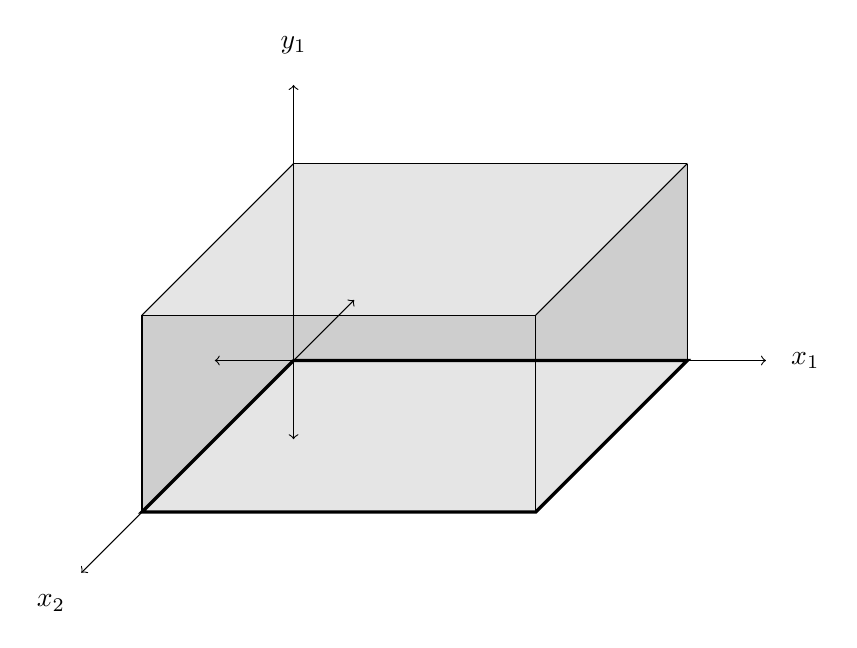
\begin{tikzpicture}
					\draw [<->] (0,0,7) -- (0,0,-2);
					\draw (0,0,8) node{$x_2$};
					\draw [<->] (-1,0,0) -- (6,0,0);
					\draw (6.5,0,0) node{$x_1$};
					\draw [<->] (0,-1,0) -- (0,3.5,0);
					\draw (0,4,0) node{$y_1$};
					\draw[very thick] (0,0,0) -- (5,0,0) -- (5,0,5) -- (0,0,5) -- (0,0,0);
					\draw (0,0,0) -- (0,2.5,0);
					\draw (5,0,0) -- (5,2.5,0);
					\draw (0,0,5) -- (0,2.5,5);
					\draw (5,0,5) -- (5,2.5,5);
					\draw (0,2.5,0) -- (5,2.5,0);
					\draw (0,2.5,0) -- (0,2.5,5);
					\draw (5,2.5,0) -- (5,2.5,5);
					\draw (0,2.5,5) -- (5,2.5,5);
					\draw [fill, opacity = 0.1] (5,0,0) -- (5,0,5) -- (5,2.5,5) -- (5,2.5,0) -- (5,0,0);
					\draw [fill, opacity = 0.1] (0,0,0) -- (0,0,5) -- (0,2.5,5) -- (0,2.5,0) -- (0,0,0);
					\draw [fill, opacity = 0.1] (0,0,0) -- (5,0,0) -- (5,2.5,0) -- (0,2.5,0) -- (0,0,0);
					\draw [fill, opacity = 0.1] (0,0,5) -- (5,0,5) -- (5,2.5,5) -- (0,2.5,5) -- (0,0,5);
				\end{tikzpicture}
				\caption{Note that the values of $\vec x$ where $\abs{\set{\vec y \st (\vec x, \vec y) \in E}} > 0$ are in bold and make up the exterior of the interval in $\R^n$. Thus for almost every $\vec x$ the set mentioned above has $\R^m$-measure zero.}
			\end{SCfigure}
		Therefore, if $h(\vec x) = \iint\ind E\, d\vec y$, it follows that $h(\vec x) = 0$ a.e. Hence, $\int h(\vec x)\, d\vec x = 0$. But also, $\iint \ind E(\vec x, \vec y)\, d\vec x\, d\vec y = \abs{E} = 0,$ as $\ind E$ clearly has $\R^{n+m}$-measure zero.\\
		
		\textit{Case 3.} Suppose that $E$ is partly open interval in $\R^{n+m}$. Then $E$ is the union of its interior and a subset of its boundary. It follows from cases 1 and 2 and (6.2) (linear combinations) that $\ind E$ has property $\cal F$.\\
		
		\textit{Case 4.} Let $E$ be an open set in $\R^{n+m}$ with finite measure. We will solve this case by breaking $E$ into countably many disjoint, partly open intervals and then use (6.3) and \textit{case 3} to prove the result. Thus write $E = \bu I_j$ where the $I_j$ are disjoint, partly open intervals as mentioned. Then, if we define $E_k = \bu_{j=1}^k I_j$, we have $\ind{E_k} = \sum_{j=1}^k \ind I$, so that $\ind{E_k}$ has property $\cal F$ by case 3 and (6.2). Therefore since $\ind{E_k} \upto \ind E$, $\ind E$ has property $\cal F$ by (6.3).\\
		
		\textit{Case 5.} This is the final cases needed to prove the lemma. Let $E$ satisfy the hypothesis of (6.4); that is, let $E$ be of $G_\delta$ with $G_1$ of finite measure. Then we may assume that $G_k \downto E$ by considering the open sets $G_1, G_1\i G_2, G_1\i G_2\i G_3, \ldots$ Then $\ind{G_k}\downto \ind E$, and the lemma follows from case 4 and (6.3).
		\end{pf}
		
	\begin{lem}{(6.5)}
		If $Z$ is a subset of $\R^{n+m}$ with measure zero, then $\ind Z$ has property $\cal F$. Hence, for almost every $\vec x \in \R^n$, the set $\set{\vec y : (\vec x, \vec y) \in Z}$ has $\R^m$-measure zero.
	\end{lem}
		\begin{pf}
			Using (3.8) | which states that for any real set, $E$, there exists a set $H$ of type $G_\delta$ such that $E \ss H$ with $\abs{H}_e = \abs{E}_e$ | we get that $Z \ss H$ and $\abs{H} = 0$. If $H = \bi G_k$, then we can assume $G_1$ has finite measure, so that by the previous theorem,
				\[ \int\left[\int\ind H(\vec x, \vec y)\, d\vec y\right]\, d\vec x = \iint \ind h(\vec x, \vec y)\, d\vec x\, d\vec y = 0. \]
			Therefore $\int \ind H(\vec x, \vec y)\, d\vec y = 0$ a.e. which implies $\abs{\vec y: (\vec x, \vec y) \in H} = 0$ for almost all $\vec x$. If $\set{\vec y : (\vec x, \vec y) \in H}$ has $\R^m$-measure zero, then so must $\set{\vec y : (\vec x, \vec y) \in Z}$ since $Z \ss H$. Therefore, as for almost every $\vec x$, $\ind Z (\vec x, \vec y)$ is measurable in $\vec y$ and $\int \ind Z (\vec x, \vec y)\, d\vec y = 0$. Hence, $\int[ \int \ind Z (\vec x, \vec y)\, d\vec y]\, d\vec x = 0$, which proves the lemma since $\iint \ind Z (\vec x, \vec y)\, d\vec x\, d\vec y = \abs{Z} = 0$.
		\end{pf}
		
	An interesting note about the previous proof, while the result seems trivial, dealing with details within integrals can be tricky. The proof therefore cleverly extends the set to a more manageable set for which we already have a theorem, and deconstructs that result to make an observation about the set itself that we can then extend back to the original set.\\
	
	\begin{lem}{(6.6)}
		Let $E\ss \R^{n+m}$. If $E$ is measurable with finite measure, then $\ind E$ has property $\cal F$.
	\end{lem}
		\begin{pf}
			The proof of this lemma follows exactly as expected. Using (3.28), we can write $E = H - Z$, where $H$ is of type $G_\delta$ and $Z$ has measure zero. IF $H = \bi G_k$, choose $G_1$ with finite measure (which is guaranteed possible by the finiteness of $E$). Since $\ind E = \ind H - \ind Z$, the lemma directly follows from (6.4), (6.5), and (6.2).
		\end{pf}
	
	Now we can prove \textbf{Fubini's theorem}.	
	\begin{pf}
		The goal is to show that every $f \in L(d\vec x\, d\vec y)$ has property $\cal F$. We can simplify this problem as $f = f^+ - f^-$, which means we can assume $f \geq 0$ and extend the result to all $f$ by (6.2). By (4.3), there are simple measurable functions $f_k\upto f$, $f_k \geq 0$. As $f_k \leq f$, $f_k \in L(d\vec x\, d\vec y)$, and by (6.3) it follows that $f$ has property $\cal F$ provided each $f_k$ does. This reduces the problem to showing that every simple measurable function has property $\cal F$.
		
		Say $f = \sum_{j=1}^N v_j\ind{E_j}$. Since each $E_j$ must have finite measure (unless $v_j$ is zero), the result follows from (6.6), which proves each $v_i\ind{E_j}$ has property $\cal F$, and (6.2) which proves their sum has property $\cal F$.
	\end{pf}
	
	From Fubini's theorem, we get that if $f \in L(\R^{n+m})$ then $f(\vec x, \vec y)$ is a measurable function of $\vec y$ for almost every $\vec x \in \R^n$. The next theorem gives a broader result where the same conclusion holds if $f$ is merely measurable. This will allow us to make a slight extension of Fubini's theorem.\\
	
	\begin{thm}{(6.7)}
		Let $f(\vec x, \vec y)$ be a measurable function on $\R^{n+m}$. Then for almost every $\vec x \in \R^n$, $f(\vec x, \vec y)$ is a measurable function of $\vec y \in \R^m$.
		
		In particular, if $E$ is a measurable subset of $\R^{n+m}$, then the set 
			\[
				E_\vec x = \set{\vec y \st (\vec x, \vec y) \in E}
			\]
		is measurable in $\R^m$ for almost every $\vec x \in \R^n$.
	\end{thm}
	\begin{pf}
		Recall that a function $f$ is measurable if $\set{f > a}$ is measurable for all $a\in\R$. We first prove the case where $f$ is the characteristic function $\ind E$ of a measurable $E\ss  \R^{n+m}$. This will also prove the particular case. We write $E = H\u Z$ where $H$ is of type $F_\sigma$ in $\R^{n+m}$ and $\abs{Z}_{n+m} = 0$. Then
			\[
				E_\vec x = \set{\vec y \st (\vec x, \vec y) \in H} \u \set{\vec y \st (\vec x, \vec y)\in Z}, \tor 
			\]
			\begin{equation*}
				E_\vec x = H_\vec x \u Z_\vec x. 
			\tag{$*$}
			\end{equation*}
		By (6.5), $\abs{Z_\vec x}_{\R^m} = 0$ for almost all $\vec x\in \R^n$. Then $H_\x$ is of type $F_\sigma$ in $\R^m$. That is, if $H = \bu F_i$ with $F_i$ closed for all $i$, then $H_\vec x = \bu F_{i_\vec x}$ and $F_{i_\vec x}$ is closed in $\R^m$. Therefore, $E_\vec x$ is measurable for almost every $\vec x$ by ($*$).
		
		Now if $f$ is any measurable function on $\R^{n+m}$, consider the set $E(a) = \set{(\vec x, \vec y): f(\vec x, \vec y) > a}$. Since $E(a)$ is measurable in $\R^{n+m}$, by the first part, the set $E(a)_\vec x = \set{\vec y \st f(\vec x, \vec y) > a}$ is measurable in $\R^m$ for almost every $\vec x \in \R^n$. The set of $\R^n$-measure zero where $E(a)_\vec x$ is not measurable depends on $a$. The union $Z$ of these exceptional sets for all rational $a$ clearly also has $\R^n$ measure zero. Recall that (4.4)  states that if $\set{f > a}$ is measurable for all $a$ in a dense subset of $\R^1$, then $f$ is measurable. Thus, if $\vec x \notin Z$ then $\set{\vec y \st f(\vec x, \vec y) > a}$ is measurable for all rational $a$; therefore, $\set{\vec y \st f(\vec x, \vec y) > a}$ is measurable for all $a$. Hence $f$ is a measurable function of $y$. 
	\end{pf}
	
	With this result we will now be able to extend Fubini's theorem to functions defined on subsets of $\R^{n+m}$. Before we go into that, however, it should be worth noting that chapter 2 was the chapter on measurable functions and it is not until chapter 6 | after we have established integration with respect to measure | that we prove that if $E$ is measurable then $E$ restricted to a smaller dimension must also be measurable. This theorem also shows us that if measurable functions are projected onto smaller dimensions, then the projections are also measurable, which is much less intuitive.
	
	\begin{thm}{(6.8)}
		Let $f(\vec x, \vec y)$ be a measurable function defined on a measurable subsest $E$ of $\R^{n=M}$, and let $E_\vec x = \set{\vec y \st (\vec x, \vec y) \in E}$.
		\bei
			\item For almost every $\vec x \in \R^n$, $f(\vec x, \vec y)$ is a measurable function of $\vec y$ on $E_\vec x$.
			\item If $f(\vec x, \vec y) \in L(E)$, then for almost every $\vec x \in \R^n$, $f(\vec x, \vec y)$ is integrable on $E_\vec x$ with respect to $\vec y$; moreover, $\int_{E\vec x} f(\vec x, \vec y) \, d\vec y$ is an integrable function of $\vec x$ and 
			\[
				\iint_E f(\vec x, \vec y)\, d\vec x\, d\vec y = \int_{\R^n} \left[ \int_{E_\vec x} f(\vec x, \vec y) \, d\vec y\right]\, d\vec x.
			\] 
		\ee
	\end{thm}
	\begin{pf}
		Let $\bar{f}$ be the function defined on $\R^{n+m}$ that is equal to $f$ on $E$ and 0 everywhere else. Since $f$ is measurable on $E$, $\bar{f}$ is measurable on $\R^{n+m}$ (as $\R^{n+m} - E$ is measurable). Therefore by (6.7), $\bar{f}(\vec x, \vec y)$ is a measurable function of $\vec y$ for almost every $\vec x\in \R^{n+m}$ | again, what we are saying here is that for almost every $\vec x \in \R^n$, the restriction of $f$ to just that value of $\vec x$ is also measurable. Since $E_\vec x$ is measurable for almost every $\vec x \in \R^n$, $\set{f > a} = \set{\bar{f} >a} \i E_x$ is also measurable for almost every $\vec x \in \R^n$. Thus $f$ is measurable on almost every $E_\vec x$ which proves (i).
		
		If $f \in L(E)$, then $\bar{f} \in L(\R^{n+m})$ and
			\[
				\iint_E f(\vec x, \vec y)\, d\vec x\, d\vec y = \iint_{\R^{n+m}} \bar{f}(\vec x, \vec y)\, d\vec x\, d\vec y = \int_{\R^n} \left[ \int_{\R^m} \bar{f}(\vec x, \vec y)\, d\vec y \right] \, d\,\vec x.
			\]
		The last equality, of course, following from Fubini's theorem. 
		
		Since $E_\vec x$ is measurable for almost every $\vec x$, we obtain by theorem (5.24) [$\int_E f = \sum_k \int_{E_k} f$ given $E = \bu_k E_k$ and $E_k$ are disjoint and measurable] that 
			\[
				\int_{\R^m} \bar{f}(\vec x, \vec y)\, d\vec y = \int_{E_\vec x}\bar{f}(\vec x, \vec y)\, d\vec y + \int_{\R^m - E_\vec x} \bar{f}(\vec x, \vec y)\, d\vec y = \int_{E_\vec x} f(\vec x, \vec y)\, d\vec y + 0
			\]
		for almost every $\vec x\in \R^n$. Part (ii) follows from combining the two equalities.
	\end{pf}
	
	To recap for (i), we expanded $f$ to $\bar{f}$ defined on all of $\R^{n+m}$, and used the previous theorem to show that this new function is measurable when projected using almost every $\vec x \in \R^n$. Then because $E_\vec x$ is measurable (also by the previous theorem) then $\bar{f}$ when restricted to $E_\vec x$ is also measurable for almost every $\vec x \in \R^n$, and of course $\bar{f}$ restricted to $E_\vec x$ is just $f$.
	
\section{Tonelli's Theorem}
	This section starts by pointing out a seemingly obvious consequence to Fubini's theorem: the finiteness of a multiple integral implies that of the corresponding iterated integrals. However, the converse of that | oddly enough | is not true. That is to say, an iterated integral could be finite byt the multiple integral could be infinite.
	
	We subdivide the two dimensional unit square into 4 quadrants and denote the bottom left quadrant as $I_1$;then subdivide the upper right quadrant and denote that bottom left quadrant as $I_2$; and so on. Now we subdivide each individual interval $I_k$ into four quadrants $I_k^{(1)}, I_k^{(2)}, I_k^{(3)}, \tand I_k^{(4)}$.
	
	Now, for each $K$, let $f = 1/\abs{I_k}$ on the first and third quadrant of $I_k$ and let $f = -1/\abs{I_k}$ on the second and fourth quadrant (ignoring the boundaries all the while). Now let $f = 0$ everywhere else on $I$; that is, the other three quadrants that we did not denote and boundaries of the subintervals. Clearly, $\int_0^1 f(x,y)\, dy = 0$ for all $x$ as projecting onto any value of $x$ either results in $f(x,y) = 0$ for all values of $y$ or $f(x,y) = 1/\abs{I_k}$ and $f(x,y) = -1/\abs{I_k}$ for the same measure of $y$. Therefore
		\[
			\int_0^1 \left[ \int_0^1 \abs{f(x,y)}\, dy \right]\, dx = \int_0^1 \left[ \int_0^1 \abs{f(x,y)}\, dx\right]\, dy = 0.
		\]
	However,
		\[
			\iint_I \abs{f(x,y)}\, dx\, dy = \sum_k \iint_{I_k} \abs{f(x,y)}\, dx\, dy = \sum_k 1 = +\infty.
		\]
		
	Hence, finiteness of the iterated integrals does not in general imply that of the multiple integral. Recall that for Fubini's theorem, we require that $f \in L(\R^{n+m})$ which eliminates the problem aforementioned, but as we try to expand Fubini's theorem to a less restrictive requirement, this is where the problem arises. In this next result, (Tonelli's theorem) we are able to drop the requirement from Fubini's theorem that $f$ have a finite integral but only by restricting $f$ to be nonnegative instead.\\
	
	\begin{thm}{(6.10)} \textbf{(Tonelli's Theorem)} Let $f(\vec x, \vec y)$ be nonnegative and measurable on an interval $I = I_1 \cross I_2$ of $\R^{n+m}$. Then, for almost every $\vec x \in I_1$, $f(\vec x, \vec y)$ is a measurable function of $\vec y$ on $I_2$. Moreover, as a function of $\vec x$, $\int_{I_1} f(\vec x, \vec y)\, d\vec y$ is measurable on $I_1$, and 
		\[
			\iint_{I} f(\vec x, \vec y)\, d\vec x\, d\vec y = \int_{I_1} \left[ \int_{I_2} f(\vec x, \vec y)\, d\vec y \right]\, d\vec x.
		\]
	\end{thm}
	\begin{pf}
		We will prove the theorem by breaking $f$ into a sequence of functions each of which is bounded and vanishes outside of a compact set. Because of this enforced restriction, each function in the sequence is integrable over $I$. This will allow us to apply Fubini's theorem to each function in the sequence and then obtain the result with the monotone convergence theorem.
		
		We start with the sequence of functions: for $k= 1,2,\ldots,$ let $f_k(\vec x, \vec y) = 0$ if $\abs{\vec x, \vec y} > k$ and $f_k(\vec x, \vec y) = \min \set{k, f(\vec x, \vec y)}$ if $\abs{(\vec x, \vec y)} \leq k$ (I assume that the norm used here is the standard norm for $\R^{n+m}$; however, it is interesting to imagine this process with an arbitrary norm). Then $f_k \geq 0$, $f_k \upto f$ on $I$ and $f_k \in L(I)$. 
	\end{pf}
	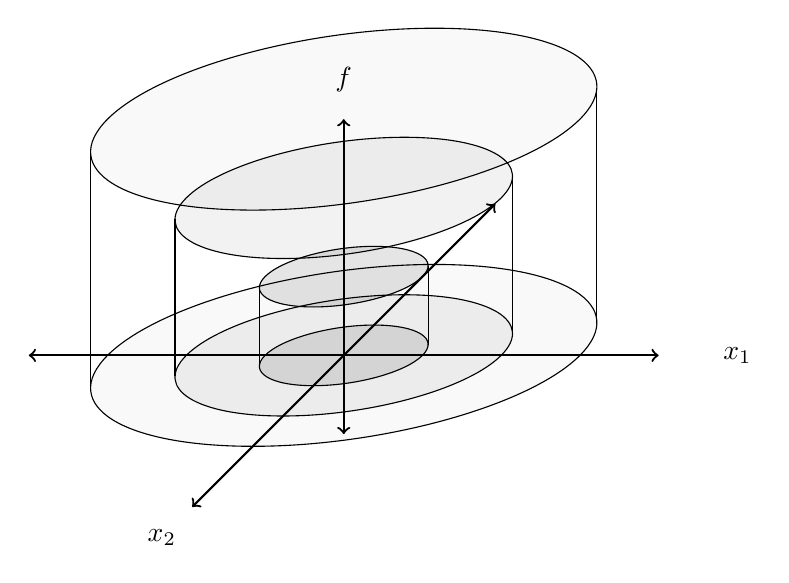
\begin{tikzpicture}
		\draw [thick, <->] (0,0,5) -- (0,0,-5);
		\draw (0,0,6) node{$x_2$};
		\draw [thick, <->] (-4,0,0) -- (4,0,0);
		\draw (5,0,0) node{$x_1$};
		\draw [thick, <->] (0,-1,0) -- (0,3,0);
		\draw (0,3.5,0) node{$f$};
		\draw ({cos(-200)},0,{sin(-200)}) -- ({cos(-200)},1,{sin(-200)});
		\draw ({cos(-20)},0,{sin(-20)}) -- ({cos(-20)},1,{sin(-20)});
		\draw ({2*cos(-200)},0,{2*sin(-200)}) -- ({2*cos(-200)},2,{2*sin(-200)});
		\draw ({2*cos(-20)},0,{2*sin(-20)}) -- ({2*cos(-20)},2,{2*sin(-20)});
		\draw ({3*cos(-200)},0,{3*sin(-200)}) -- ({3*cos(-200)},3,{3*sin(-200)});
		\draw ({3*cos(-20)},0,{3*sin(-20)}) -- ({3*cos(-20)},3,{3*sin(-20)});
		\begin{scope}[canvas is xz plane at y=0]
			\draw (0,0) circle (1);
			\draw[fill, opacity=0.1] (0,0) circle (1);
			\draw (0,0) circle (2);
			\draw[fill, opacity=0.05] (0,0) circle (2);
			\draw (0,0) circle (3);
			\draw[fill, opacity=0.025] (0,0) circle (3);
		\end{scope}
		\begin{scope}[canvas is xz plane at y=1]
			\draw (0,0) circle (1);
			\draw[fill, opacity=0.1] (0,0) circle (1);
		\end{scope}
		\begin{scope}[canvas is xz plane at y=2]
			\draw (0,0) circle (2);
			\draw[fill, opacity=0.05] (0,0) circle (2);
		\end{scope}
		\begin{scope}[canvas is xz plane at y=3]
			\draw (0,0) circle (3);
			\draw[fill, opacity=0.025] (0,0) circle (3);
		\end{scope}
	\end{tikzpicture}

\chapter{Differentiation}
\chapter{$\bf{L^p}$ Classes}


\end{document}